\chapter{Evaluation}
\label{sec:evaluation}

% Zu jeder Arbeit in unserem Bereich gehört eine Leistungsbewertung. Aus
% diesem Kapitel sollte hervorgehen, welche Methoden angewandt worden,
% die Leistungsfähigkeit zu bewerten und welche Ergabnisse dabei erzielt
% wurden. Wichtig ist es, dem Leser nicht nur ein paar Zahlen
% hinzustellen, sondern auch eine Diskussion der Ergebnisse
% vorzunehmen. Es wird empfohlen zunächst die eigenen Erwartungen
% bezüglich der Ergebnisse zu erläutern und anschließend eventuell
% festgestellte Abweichungen zu erklären.
In previous chapters, we analyzed the security issues of the upstream quark in confidential computing, and proposed the design and implementation of Confidential Quark as a countermeasure. In this chapter, we evaluate the security and performance of Confidential Quark from both 
qualitative and quantitative perspectives.
\begin{figure}[H]
    \centering
    \begin{subfigure}[b]{0.45\textwidth}
        \centering
        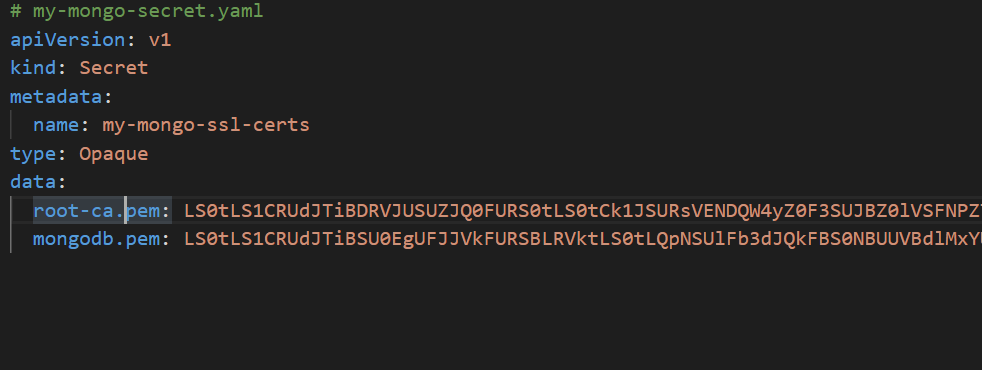
\includegraphics[width=\textwidth]{images/mongo_secret.PNG}
        \caption{YAML file for deploying K8s secret}
        \label{fig:mongo_secret}
    \end{subfigure}
    \hfill
    \begin{subfigure}[b]{0.45\textwidth}
        \centering
        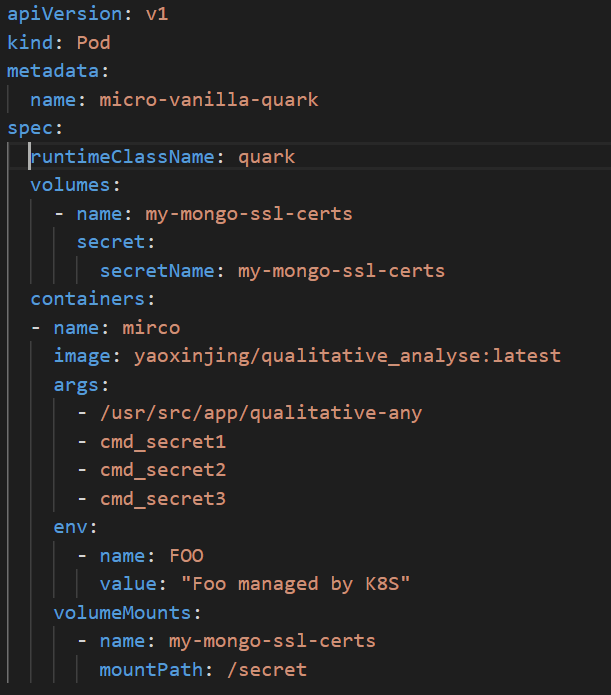
\includegraphics[width=\textwidth]{images/vanila_quark_deployment.PNG}
        \caption{YAML file for deploying application in vanilla quark}
        \label{fig:vanila_quark_deployment}
    \end{subfigure}
    \hfill
       \caption[Artifacts for deploying applications in Vanilla Quark]{Artifacts for deploying applications in Vanilla Quark. The YAML file on the left is used to submit the Kubernetes secret with the name my\-mongo\-ssl\-certs to the cluster. 
       This secret includes two files, namely root\-ca.pem and mongodb.pem. Meanwhile, the YAML file on the right on the right is used to deploy application. This file passes three command line secrets, namely cmd\_secret1\-3, an environment variable secret named FOO, and mounts the 
       Kubernetes secret (file type secret) to the secret directory of the application rootfs.}
       \label{fig:three graphs}
\end{figure}
\section{Qualitative Analysis}
In this section, we provide a synopsis of the security vulnerabilities uncovered during the security analysis in Chapter 3, targeting the vanilla quark environment. Furthermore, we detail our implementation strategies for addressing these vulnerabilities.

\subsection{Common Setup}

This section provides an overview of the common configuration for the analysis. Firstly, we set up the Confidential Quark and vanilla Quark environments following the guidelines presented in the Quark demo repository\cite*{Qaurk_Demo_for_qualitativ}.
These include creating the Kubernetes cluster and compiling securectl, confidential quark, and key broker service. To deploy a vanilla quark-based application, we need to upload the Kubernetes secret\cite*{k8s_secret_yaml} in Figure ~\ref{fig:mongo_secret} and use 
the YAML file\cite*{vanilla_quark_deploy_for_qualitativ_yaml} (~\ref{fig:vanila_quark_deployment}). 


\begin{figure}[H]
    \centering
    
    \begin{minipage}{0.9\textwidth}
    \begin{subcolumns}[0.62\textwidth]
      \subfloat[YAML file for deploying application\label{fig:c_quark_deployment}]{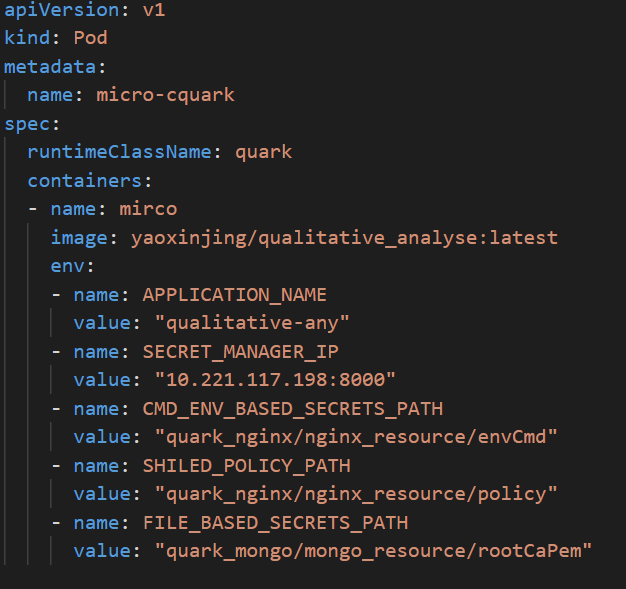
\includegraphics[width=\subcolumnwidth]{images/c_quark_deployment.PNG}}

    \nextsubcolumn[0.33\textwidth]
      \subfloat[KBS managed file type secret\label{fig:file_secrets}]{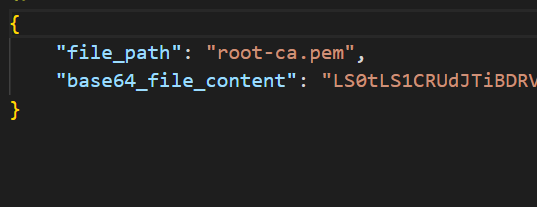
\includegraphics[width=\subcolumnwidth]{images/file_secrets.PNG}}

    \nextsubfigure
      \subfloat[KBS managed cmd \&\& envv type secrets\label{fig:cmd_env_secrets}]{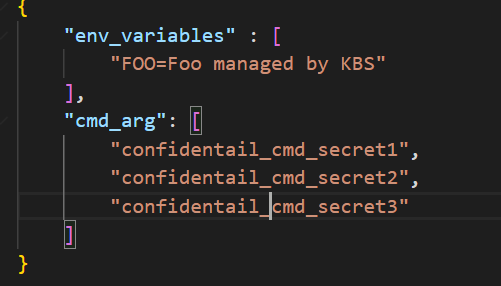
\includegraphics[width=\subcolumnwidth]{images/cmd_env_secrets.PNG}}
    \end{subcolumns}
    \end{minipage}
    
    \caption[The artifacts used to deploy the application in Confidential Quark]{The artifacts used to deploy the application in Confidential Quark. Figures ~\ref{fig:file_secrets} and ~\ref{fig:cmd_env_secrets} show the file type secret root\-ca.pem, as well as the environment variables, and the command line type secret managed by kbs. The YAML in Figure  is
    a utilized to deploy the application in cquark. In this file, we specify the IP address of KBS, and the URL for enclave to fetch the secrets and enclave policy from KBS. The enclave can use the above information to establish a secure channel with the KBS and 
    deploy the secret to the application process.}
    \label{fig:cquark_deployment}
\end{figure}


The enclave policy file\cite*{enclave_policy} in Figure ~\ref{fig:generic_policy}, fsecrets in Figures ~\ref{fig:file_secrets}  and ~\ref{fig:cmd_env_secrets} \cite*{kbs_secret}, and the YAML file\cite*{confidentail_quark_yaml} in Figure ~\ref{fig:c_quark_deployment}  are used for 
application deployment in confidential quark. 
\begin{figure}[H]
    \centering
    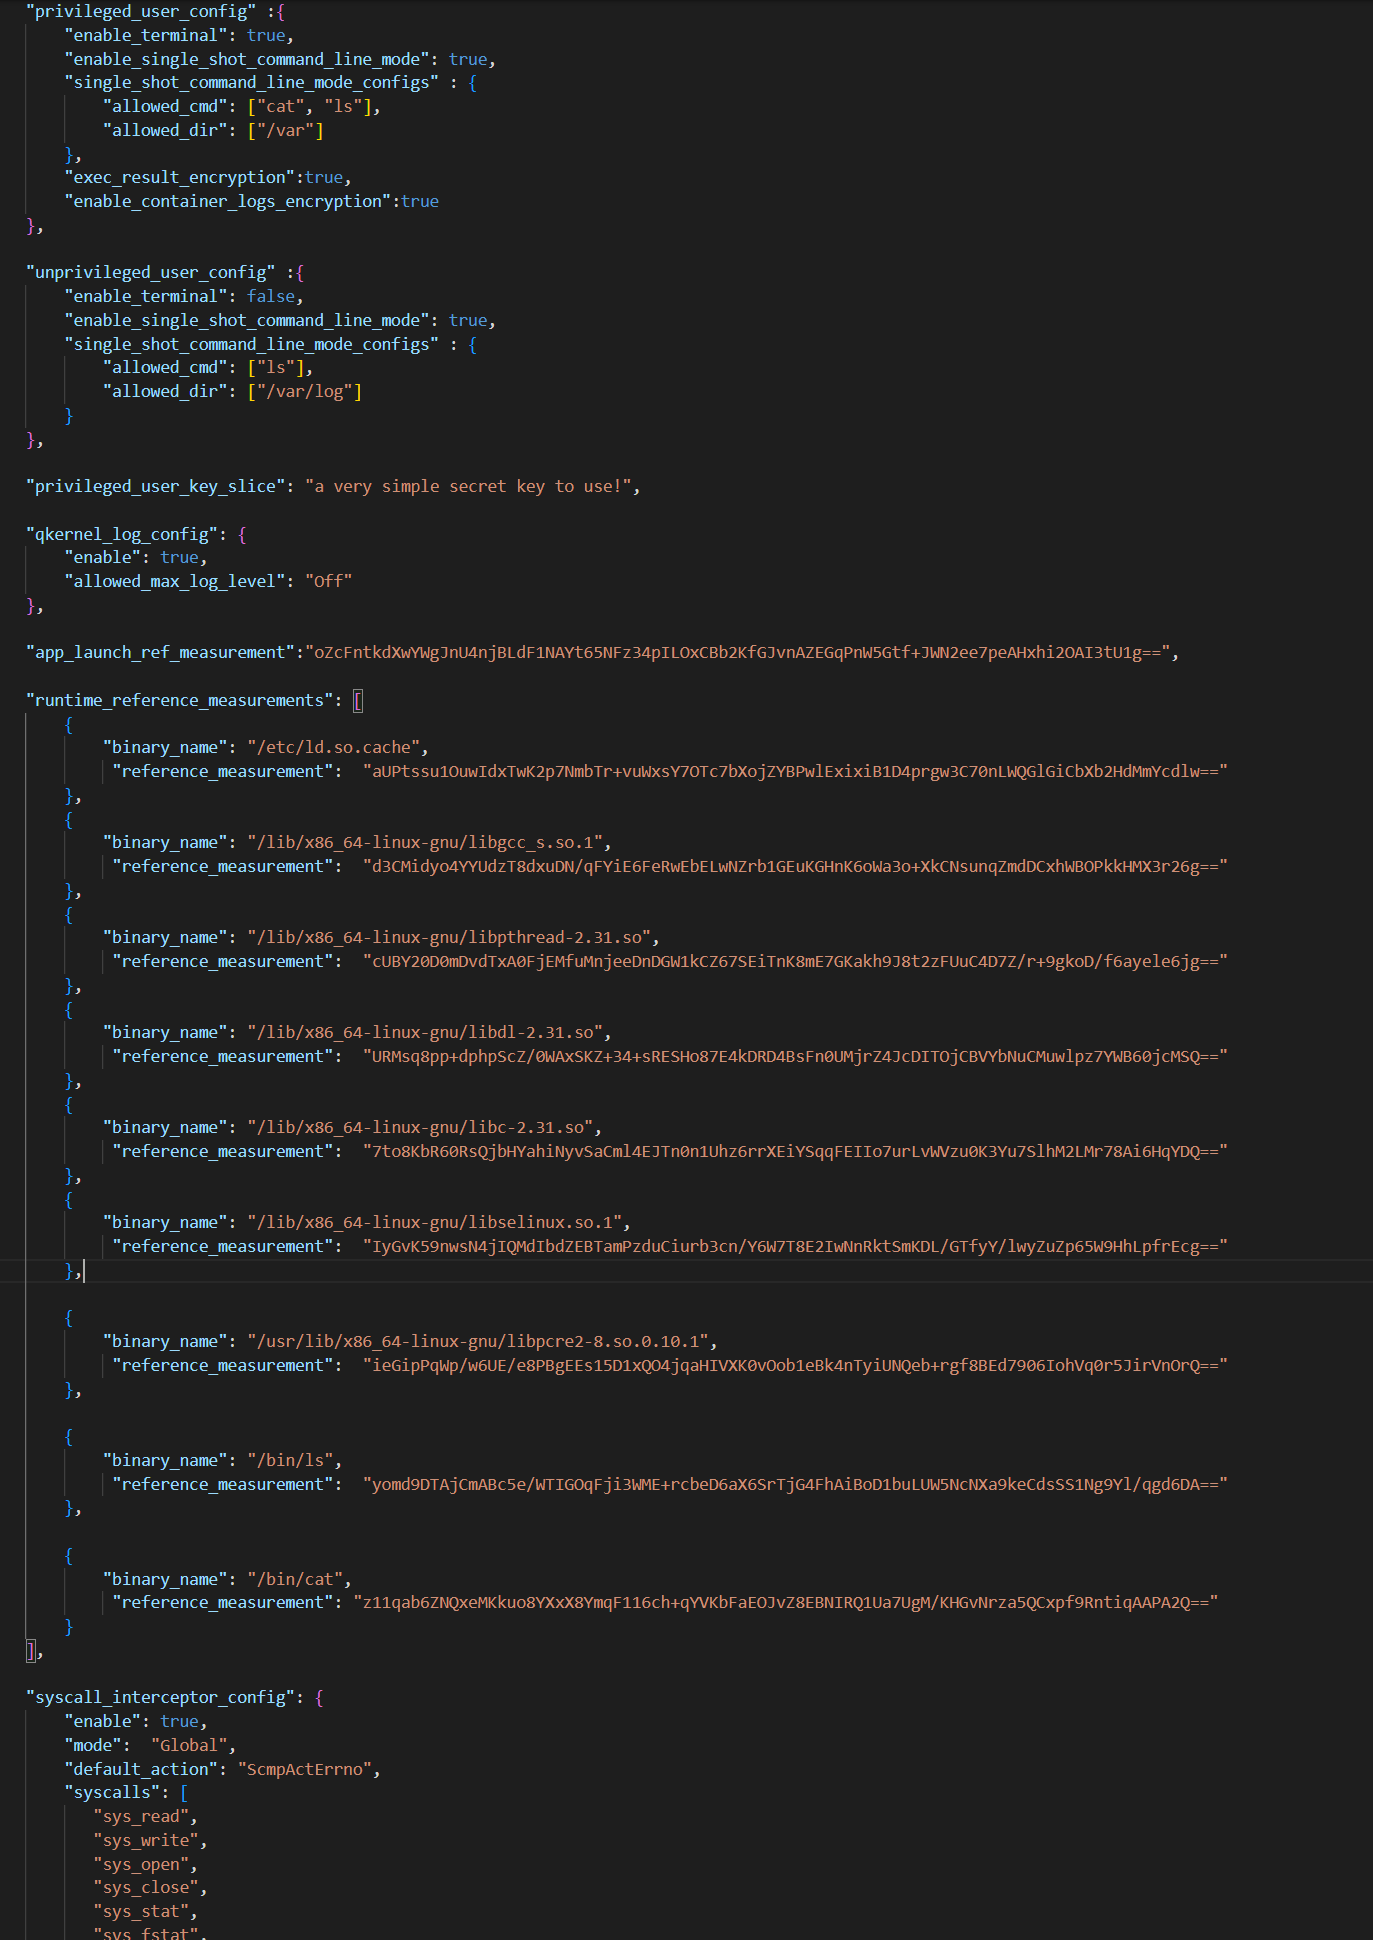
\includegraphics[width=0.8\textwidth, scale=0.8]{images/generic_policy.PNG}
    \caption[Qkernel Attestation Report Syscall Benchmark Deployment]{The shield policy used by the enclave.  The policy is uploaded to the Key Broker Service (KBS) by enclave owner. KBS verifies the integrity of the enclave's runtime environment 
    using the hash in app{\_}lauch{\_}ref{\_}measurment and sends the policy to the enclave securely. The policy stipulates that enclave is in production mode, in which the enclave use the hash from runtime\_reference\_measurements to validate the 
    integrity of the binaries and dynamic link libraries loaded from host at application runtime. The policy also permits privileged users to create terminals and issues cat and ls commands, alongside cryptographic protection for the results 
    of the commands and application logs (see privileged{\_}user{\_}config). Conversely, non{\-}privileged users' allocation of terminals is blocked, and they can only issue ls commands (refer to the option unprivileged{\_}user{\_}config). The option 
    qkernel\_log\_config in policy further enables the qkernel's logging system interceptor, while the logging level is Off, resulting in no output from the log system. Lastly, the guest system call interceptor is activated, and the policy configures 
    it to global mode (syscall{\_}interceptor{\_}config). N.b., the white list "syscall" contains 0-451 system calls, some of which are excluded from the figure due to space constraints.}
    \label{fig:generic_policy}
\end{figure}
\todo{update the policy file,  enclave mode is missing, change the system call to ContextBased}
Notably, for the following demonstration, Confidential quark commit \cite*{qualitativ_confidentail_quark} and vanilla quark commit \cite*{qualitativ_baseline} are utilized, and the policy\cite*{enclave_policy} (Figure ~\ref{fig:generic_policy}) and application\cite*{qualitativ_workload} (Figure ~\ref{fig:analysis_workload}) are used by default unless stated otherwise. As the application is already containerized, 
we deploy it to either the cquark or vanilla quark environment using the YAML files in Figures ~\ref{fig:c_quark_deployment} and ~\ref{fig:vanila_quark_deployment}, respectively.  All artifacts related to the demo experiments covered in subsequent subsections are uploaded to GitHub\cite*{Qaurk_Demo_for_qualitativ}.



\begin{figure}[H]
    \centering
    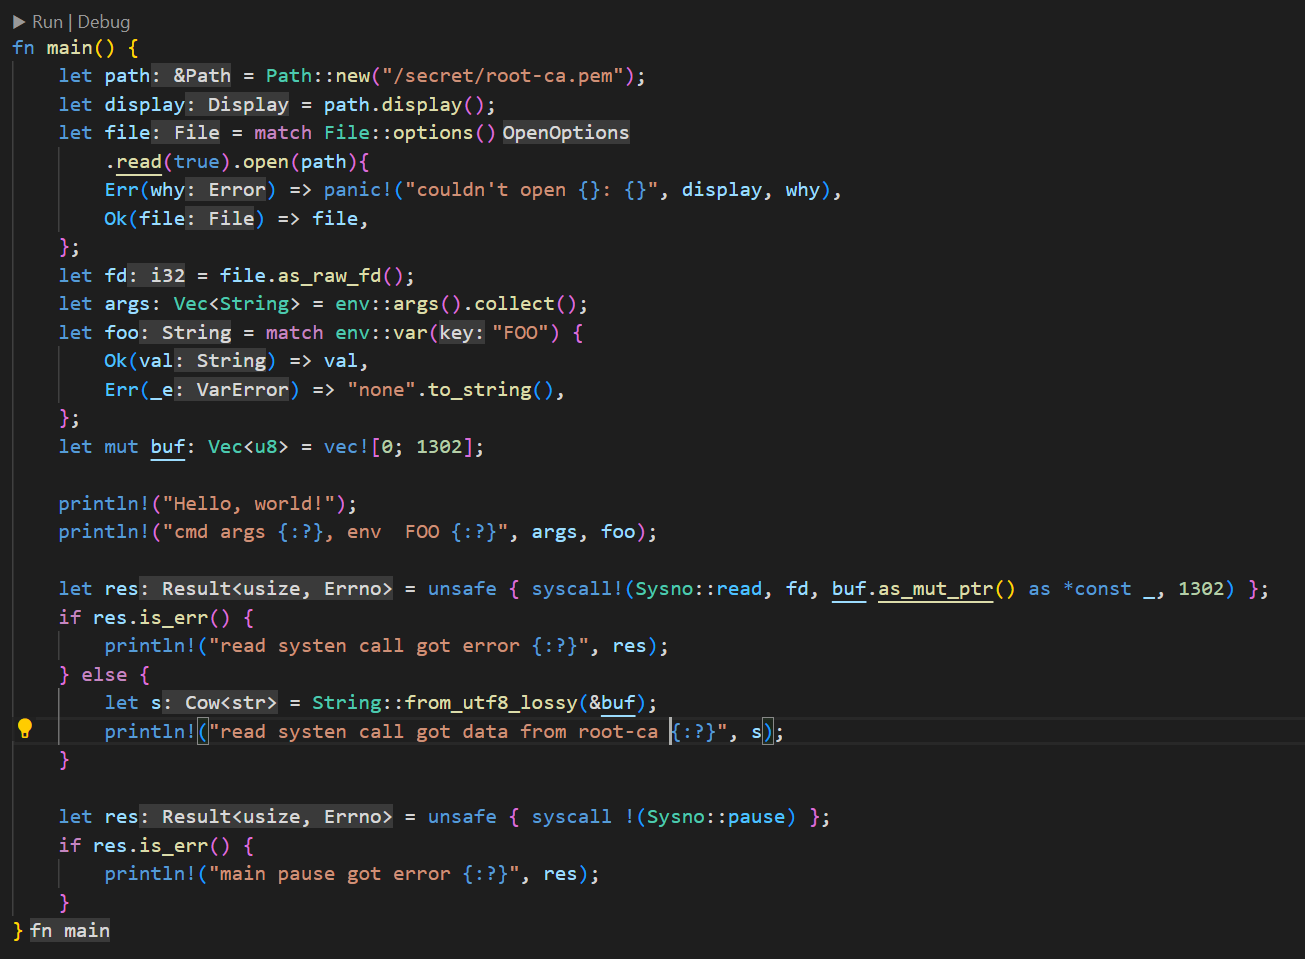
\includegraphics[width=0.8\textwidth]{images/analysis_workload.PNG}
    \caption[Sample program for demo in qualitative analysis]{Sample program for demo in qualitative analysis. This program outputs "hello world", command line arguments, and the environment variable "foo" to the standard output while also attempting to read the secret "root-ca.pem" under the directory "/secret"}
    \label{fig:analysis_workload}
\end{figure}



\subsection{Deploying Secrets via untrusted Entities (Kubelet, Containerd, Qvisor)}


Vanilla Quark benefits from Kubernetes\cite*{k8s} to manage and deploy secrets. This involves submitting three types of secrets i.e., file type, command line type, and environment variable type secrets to the Kubernetes through YAML files. Subsequently, Kubernetes offers the ability to effortlessly 
pass these secrets to the application at the time of container creation.  An example of deploying application in vanilla enviroment is displayed in Figure ~\ref{fig:vanilla_quark_deployment_result}.

\begin{figure}[H]
    \centering
    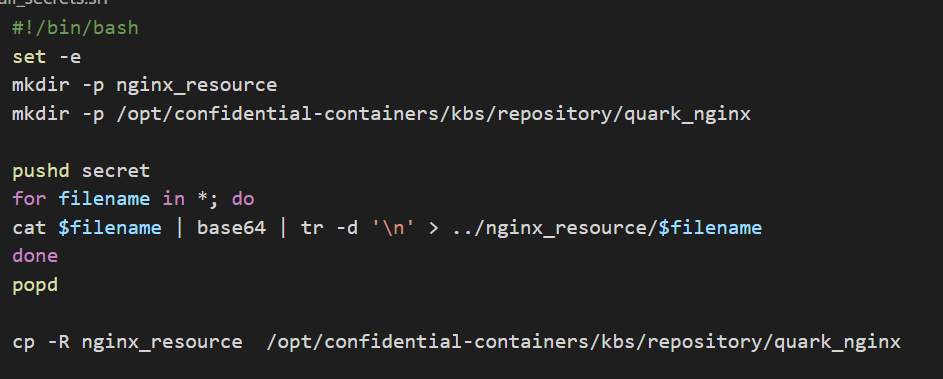
\includegraphics[width=0.8\textwidth]{images/kbs_secret_deployment.png}
    \caption[Shell script for deploying secret to KBS’s localfs backend]{Shell script for deploying secret to KBS’s localfs backend}
    \label{fig:kbs_secret_deployment}
\end{figure}

For instance, here, we use YAML file in Figure ~\ref{fig:mongo_secret} to submit the file type secret to Kubernetes, and the YAML file in Figure  ~\ref{fig:vanila_quark_deployment} to submit the command line type and environment variable type secrets as well as deploying the application. 
Our results, described in Figure ~\ref{fig:vanilla_quark_deployment_result}, illustrate that the program deployment is successful.  The command-line and environment variable secrets are appropriately printed to the standard output, while the file-type secret are securely mounted under  
“secret” directory in the application’s rootfs on the host (~\ref{fig:vanilla_quark_deployment_result_file_secret_mount_location}). 

\begin{figure}[H]

    \subfloat[Application deployment process in vanilla quark\label{fig:vanilla_quark_deployment_result}]{%
      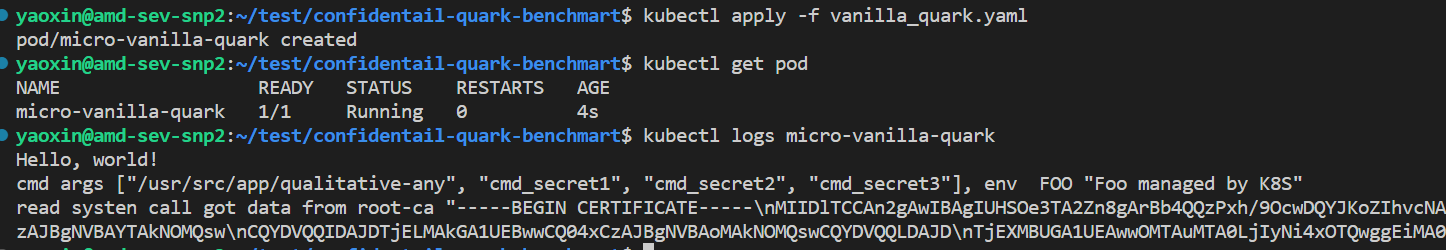
\includegraphics[clip,width=\columnwidth]{images/vanilla_quark_deployment_result.png}%
    }
    
    \subfloat[The way Kubernetes manages and deploys file type secrets\label{fig:vanilla_quark_deployment_result_file_secret_mount_location}]{%
      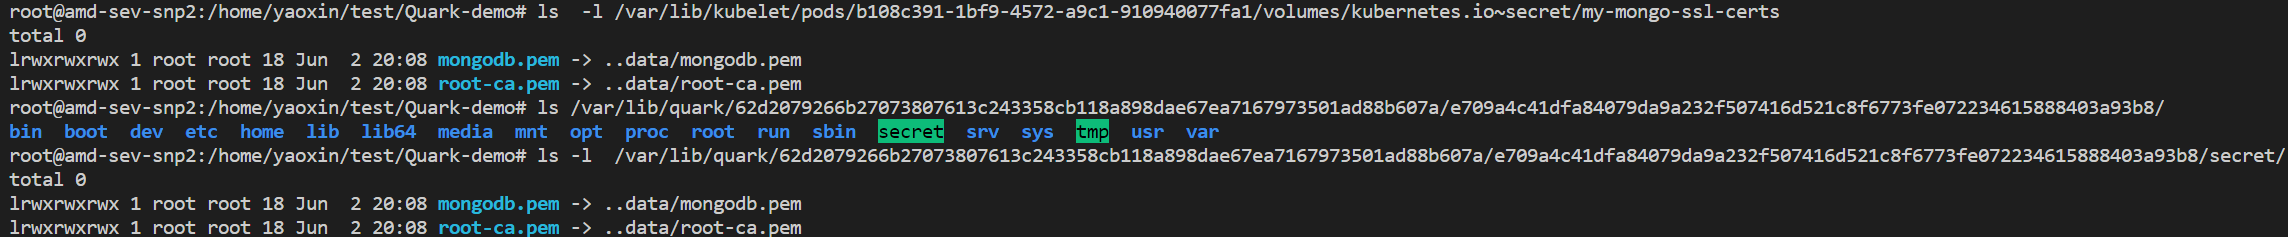
\includegraphics[clip,width=\columnwidth]{images/vanilla_quark_deployment_result_file_secret_mount_location.png}%
    }
    
    \caption{The process of deploying the application in the vanilla quark environment and its results. Figure ~\ref{fig:vanilla_quark_deployment_result} demonstrates the deployment method, wherein an application is deployed using the YAML in Figure ~\ref{fig:vanila_quark_deployment}, and illustrates the program successfully retrieves and 
    prints the command\-line types, environment variable types, and file-type secrets from k8s. Figure ~\ref{fig:vanilla_quark_deployment_result_file_secret_mount_location} reveals that k8s manages the submitted k8s secret (See figure ~\ref{fig:mongo_secret} ) in the /var/lib/kubelet directory of 
    the host machine and mounts it to the rootfs of the application on the host under var/lib/quark}
    
\end{figure}
However, managing and deploying secrets by Kubernetes compromise applications’ confidentiality, because  Kubernetes is not a trusted entity. To address this, in confidential quark, we have shifted such responsibility from Kubernetes to the Key Broker Service (KBS), which managing secrets and 
securely injects required secrets directly into an enclave. Ideally, the secret owner must attest kbs and upload the secret to it securely. Regrettably, due to time constraints, this feature is yet to be implemented. To this end, we utilize the script in Figure ~\ref{fig:kbs_secret_deployment} to 
deploy the secrets in Figures ~\ref{fig:file_secrets} and ~\ref{fig:cmd_env_secrets} onto the designated location on the local file system. During runtime, KBS extracts the secret from this location and employs secure channels to securely transmit it over to the enclave. The application deployment 
process in the CQuark environment, along with its results, is displayed in Figure ~\ref{fig:cquark_deployment_result_file_secret_mount_location}.
\begin{figure}[H]

    \subfloat[Application deployment process in confidential quark\label{fig:cquark_deployment_result}]{%
      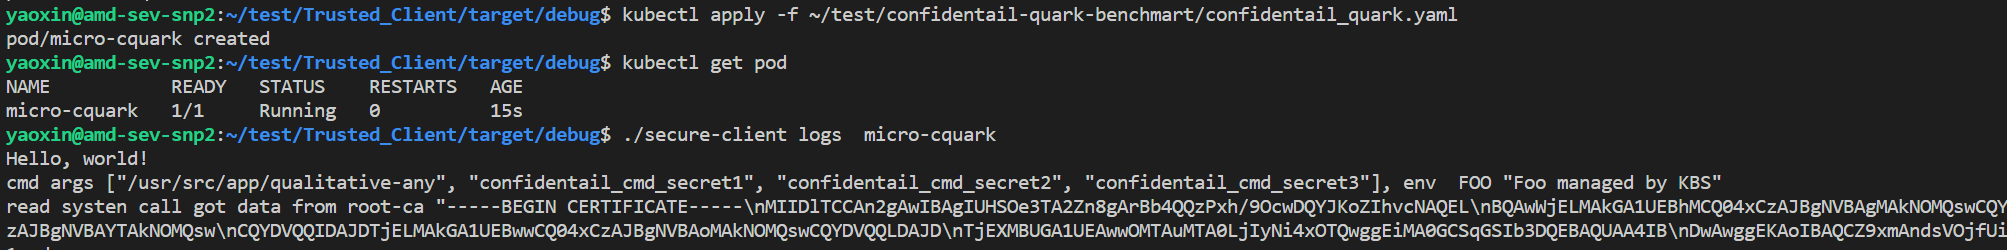
\includegraphics[clip,width=\columnwidth]{images/cquark_deployment_result.PNG}%
    }
    
    \subfloat[The way enclave manages the file type secrets\label{fig:cquark_deployment_result_file_secret_mount_location}]{%
      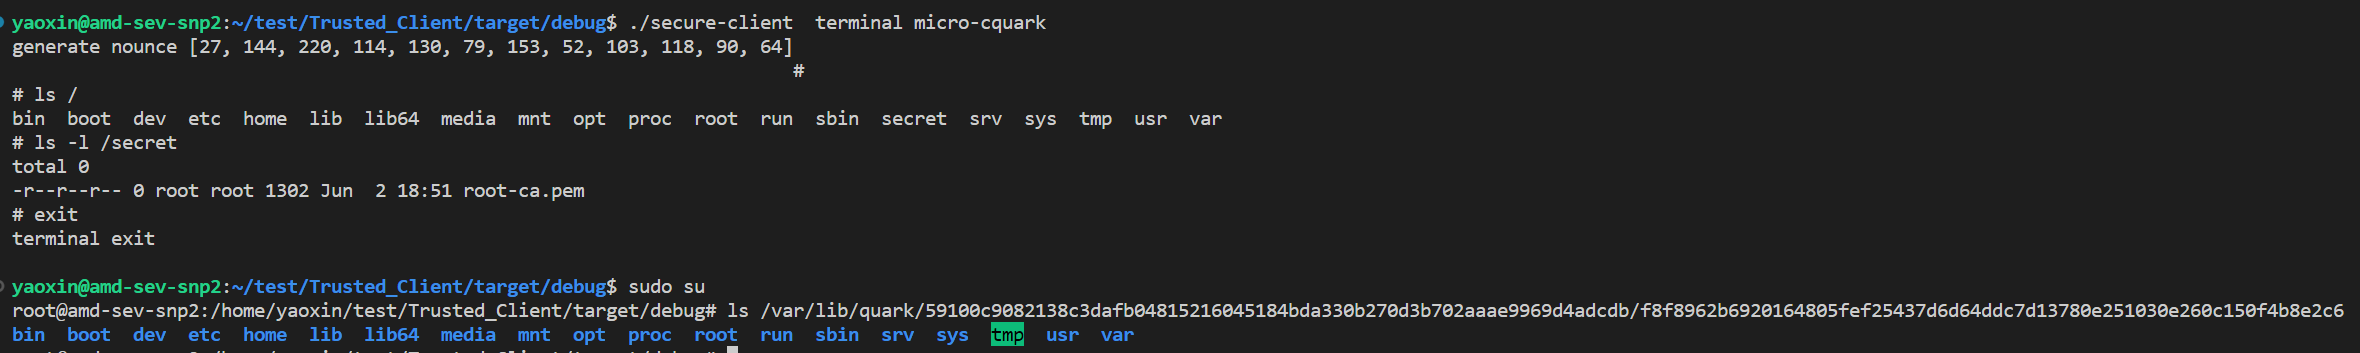
\includegraphics[clip,width=\columnwidth]{images/cquark_deployment_result_file_secret_mount_location.png}%
    }
    
    \caption[The process of deploying the application in confidential Quark environment and its results.]{The process of deploying the application in confidential Quark environment and its results. Figure ~\ref{fig:cquark_deployment_result} illustrates the deployment method, wherein an application is deployed using the YAML file in Figuer ~\ref{fig:c_quark_deployment},  
    and shows that the program successfully retrieves and prints the command-line types, environment variable types, and file\-type secrets from KBS. In Figure ~\ref{fig:cquark_deployment_result_file_secret_mount_location} , we first use securectl to allocate a terminal inside the enclave and view the file type secret located in the /secret directory. 
    We can see that the secret root-ca.pem is stored in the /secret. We then exite the terminal and exam the rootfs of the application on the host, which showed that the secret directory is not visible on the host side.}
\end{figure}


Regarding file-type secrets, as detailed in Chapter 5, the enclave retains the file-type secret on guest memory and establishes a guest sub-file system under the /secret directory. This file system enables applications to access file-type secrets. Notably, because both the file system and secret 
files exist only inside the enclave, the directory and its contents remain invisible to the application rootfs on the host (see Figure ~\ref{fig:cquark_deployment_result_file_secret_mount_location}). Consequently, secrets remain inaccessible to attackers who attempt to acquire them by 
investigating the application rootfs on the host.


\subsection{Executing arbitrary command in container}
In vanilla quark, anyone can execute commands on an application without any restrictions, thereby posing a potential risk to the confidentiality of the application.  For instance, If the application stores confidential information under the /var/log path, an attacker could use the "cat" 
command to view the unauthorized file content (see figure ~\ref{fig:vanila_execute_cat_cmd}).


\begin{figure}[H]
    \centering
    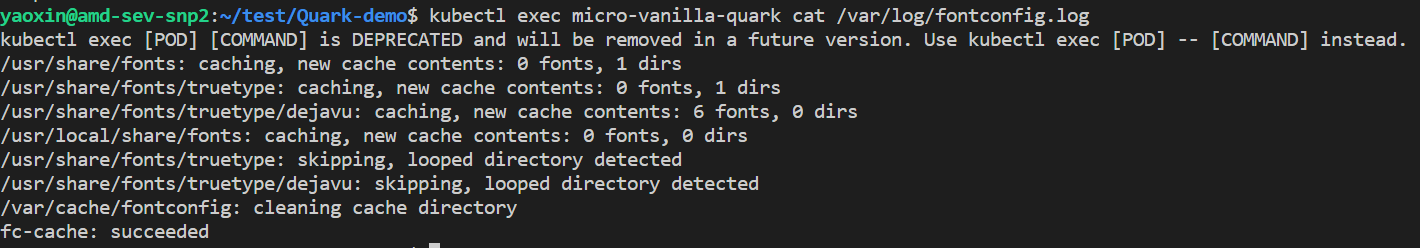
\includegraphics[width=1\textwidth]{images/vanila_execute_cat_cmd.png}
    \caption[Issues a cat command to the program running in vanilla quark]{Issues a cat command to the program running in vanilla quark.}
    \label{fig:vanila_execute_cat_cmd}
\end{figure}


Confidential quark addresses this issue by categorizing commands into two: unprivileged user commands issued by kubectl and privileged user commands issued by securectl. Here, unprivileged users refer to untrusted entities such as the cluster operator, 
whereas privileged users are specifically defined as application owner. Confidential quark empowers the application owner to establish a shield/enclave policy, which outlines the allowed commands for non-privileged users and the directories where the commands can run. 
In Figure ~\ref{fig:cuqark_unprivileged_user_cat_rejected}, the attacker's attempt to issue the cat command using kubectl is refused because the shield policy prohibits unprivileged users from issuing cat commands (refers to the option single\_shot\_command\_line\_mode\_configs of 
unprivileged user config in policy ~\ref{fig:generic_policy} ).

\begin{figure}[H]
    \centering
    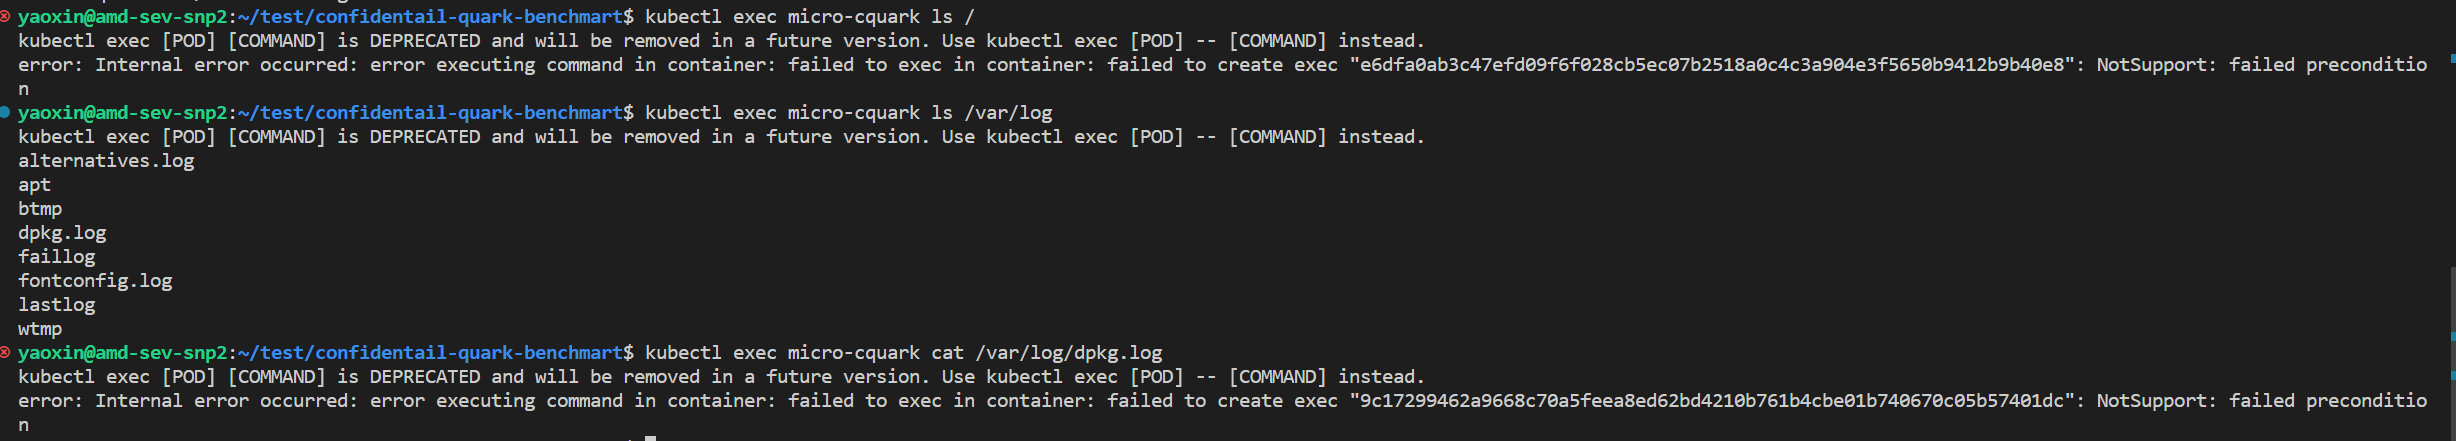
\includegraphics[width=1\textwidth]{images/cuqark_unprivileged_user_cat_rejected.png}
    \caption[Use Kubectl to issue unprivileged commands to programs running in confidential quark]{Use Kubectl to issue unprivileged commands to programs running in cquark.  The attempt to execute non-privileged commands "ls /" and "cat /var/log/dpdk" is met with rejection by Cquark. 
    The "ls /" command is disallowed as the enclave policy prohibits the execution of any unprivileged commands in the root directory, while "cat /var/log/dpdk" was rejected as it is not included in the unprivileged command whitelist (the option single\_shot\_command\_line\_mode\_configs of 
    unprivileged user config in policy ~\ref{fig:generic_policy}) }
    \label{fig:cuqark_unprivileged_user_cat_rejected}
\end{figure}

Instead, as shown in Figure ~\ref{fig:cuqark_privileged_user_cat_allowed}, the application owner is allowd to send a cat command to the enclave and view the contents of file /var/log/dpkg.log.

\begin{figure}[H]
    \centering
    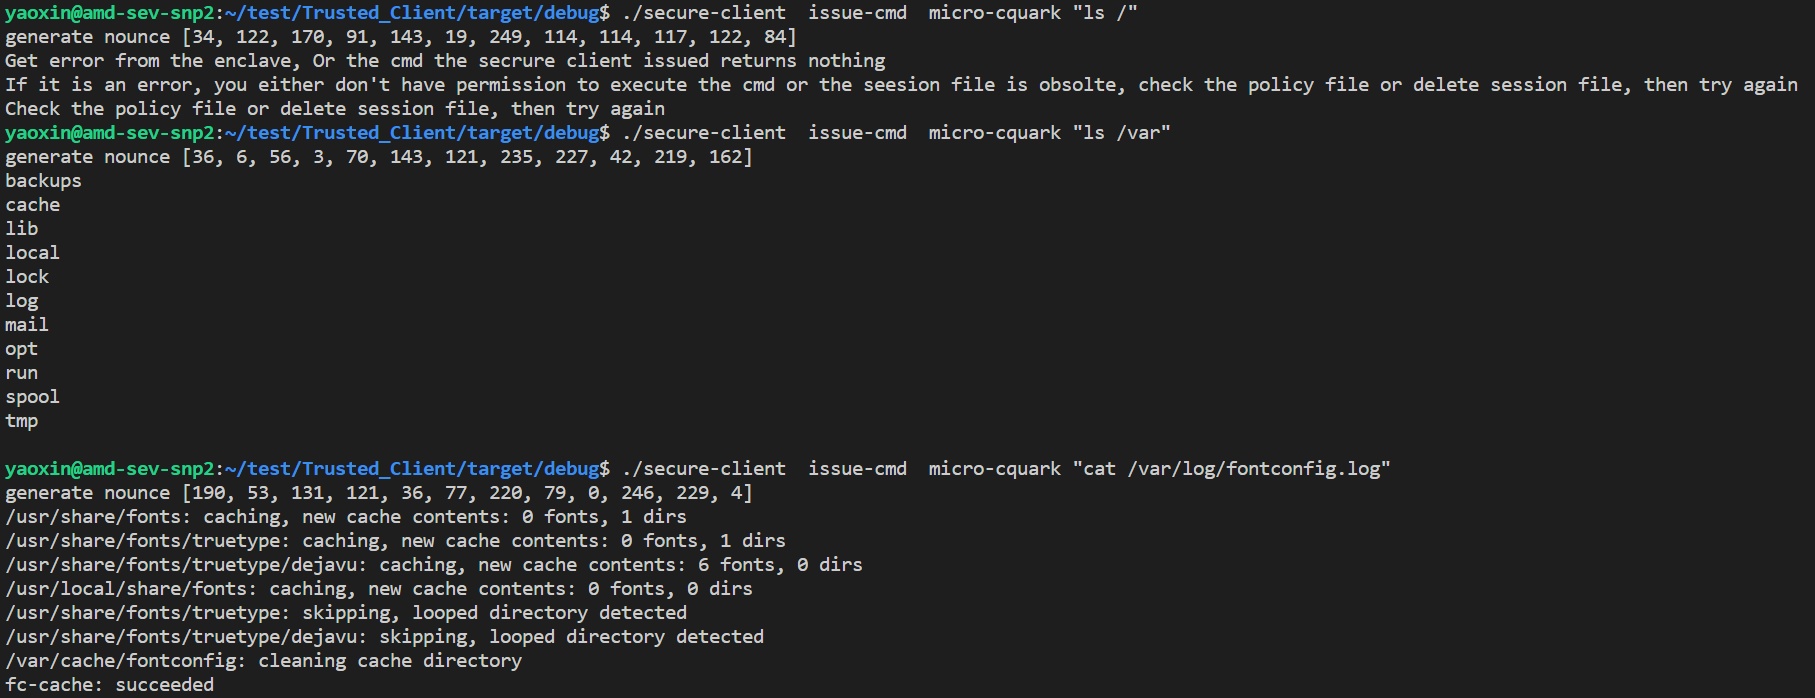
\includegraphics[width=1\textwidth]{images/cuqark_privileged_user_cat_allowed.png}
    \caption[Use Securectl to issue privileged commands to programs running in cquark]{Use Securectl to issue privileged commands to programs running in cquark.  The "ls /" command is rejected as the enclave policy prohibits the execution of any privileged commands in the root directory 
    , while "cat /var/log/dpdk" and ls /var are allowed because ls and cat are in the privileged command whitelist and the directories "/var" and "/var/log" are within the range of directories that are allowed to execute privileged commands (option single\_shot\_command\_line\_mode\_configs of 
    privileged user config in policy ~\ref{fig:generic_policy}).}
    \label{fig:cuqark_privileged_user_cat_allowed}
\end{figure}


Additionally, to prevent attackers from executing commands by allocating a terminal in the application, we prohibit non-privileged users from creating a terminal using kubectl by setting enable\_terminal to fasle in unprivileged user config section in the policy ~\ref{fig:generic_policy}. 
However, privileged users can still create a terminal by using securectl, as the enable\_terminal of privileged user config in policy ~\ref{fig:generic_policy} remains enabled (Figuer ~\ref{fig:cquark_terminal}).

\begin{figure}[H]
    \centering
    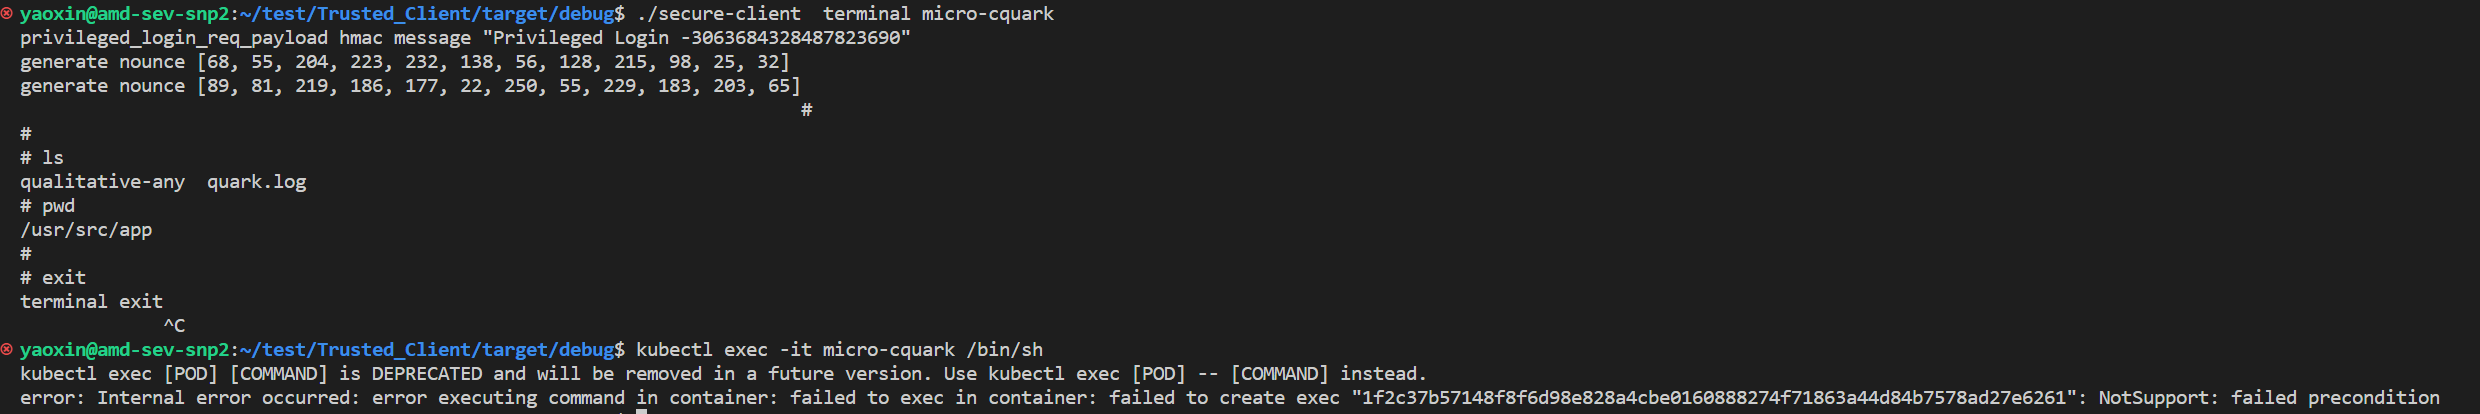
\includegraphics[width=1\textwidth]{images/cquark_terminal.png}
    \caption[Attempting to allocate a terminal through both securectl and kubectl]{Attempting to allocate a terminal through both securectl and kubectl。The request from kubectl is rejected because the enclave policy only allows privileged users to spawn a terminal using securectl 
    (option enable\_terminal of unprivileged/privileged user config in policy ~\ref{fig:generic_policy})}
    \label{fig:cquark_terminal}
\end{figure}

The outcome of the privileged command may contain confidential data. As this data is transmitted via Kubernetes\cite*{k8s} - an untrusted entity - the enclave encrypts it to ensure its protection from unauthorized access. After the encrypted execution result is returned to securectl, it decrypts it 
using the key shared between itself and enclave (option privileged\_user\_key\_slice in policy ~\ref{fig:generic_policy}). This process is depicted in Figuer ~\ref{fig:cquark_priviled_cmd_result_protection}.

\begin{figure}[H]
    \centering
    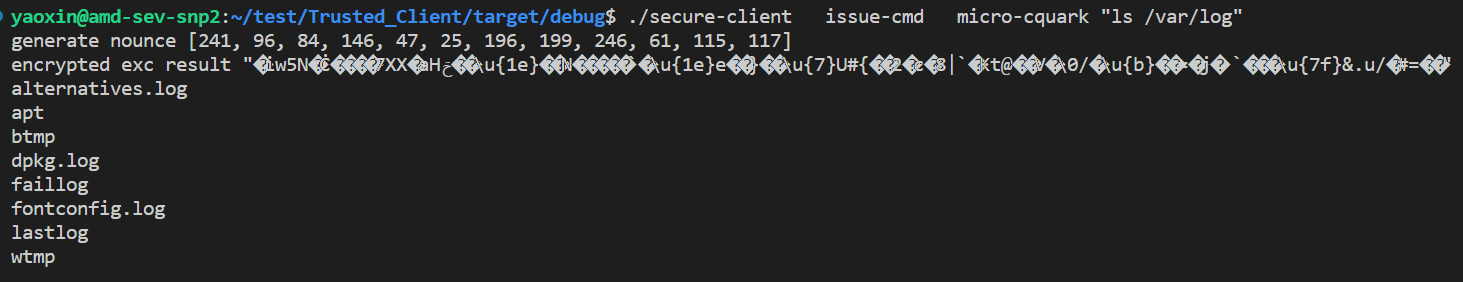
\includegraphics[width=1\textwidth]{images/cquark_priviled_cmd_result_protection.png}
    \caption[Process for securectl to handle privileged level commands]{Process for securectl to handle privileged level commands. This includes decrypting, verifying the integrity of the returned data, and printing the result}
    \label{fig:cquark_priviled_cmd_result_protection}
\end{figure}

\subsection{Application log in plaintext managed by untrusted entity}
Vanilla Quark allows any user to access the application log messages via kubectl log\cite*{kubectl} (see Figure ~\ref{fig:vanilla_queak_app_log}). 
Yet, these log messages may contain sensitive data of an application.
\begin{figure}[H]
    \centering
    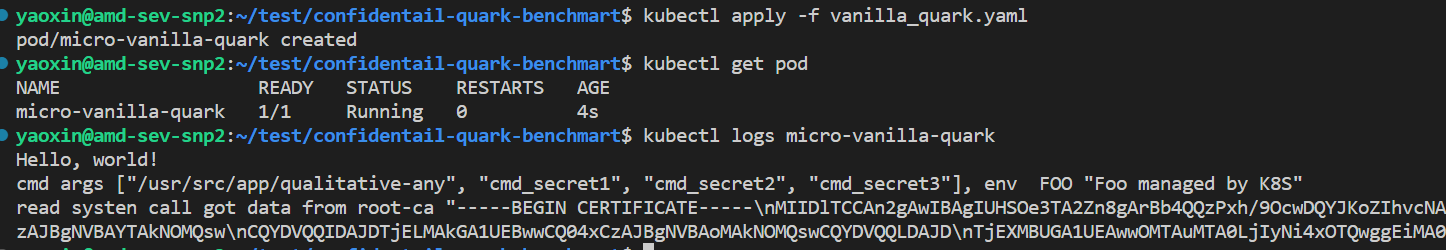
\includegraphics[width=1\textwidth]{images/vanilla_queak_app_log.png}
    \caption[Accessing application log using kubectl in vanilla quark environment]{Accessing application log using kubectl in vanilla quark environment}
    \label{fig:vanilla_queak_app_log}
\end{figure}

To prevent attackers from accessing the application log through kubectl log\cite*{kubectl}, the enclave in confidential quark encrypts the application logs. Thus, only privileged users, namely the application owners, can view the logs by using securectl (as shown in Figure ~\ref{fig:cquark_log_from_secure_ctl}).
 On the other hand, non-privileged users who use kubectl log can only access the logs in ciphertext (as depicted in Figure ~\ref{fig:cquark_log_from_kubectl}).

\begin{figure}[H]

    \subfloat[Accessing application log using securectl in confidential quark\label{fig:cquark_log_from_secure_ctl}]{%
      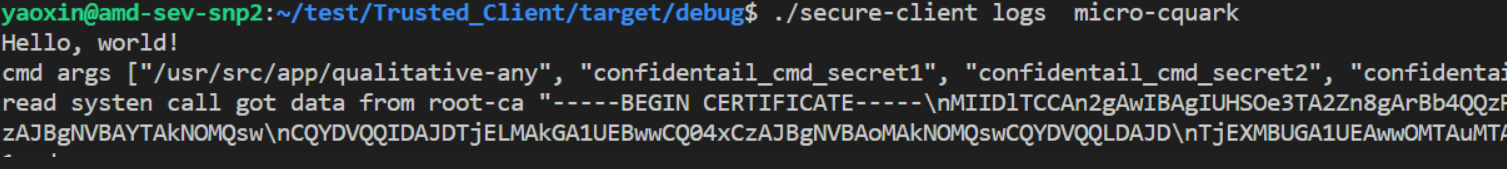
\includegraphics[clip,width=\columnwidth]{images/cquark_log_from_secure_ctl.png}%
    }
    
    \subfloat[Accessing application log using kubectl in confidential quark\label{fig:cquark_log_from_kubectl}]{%
      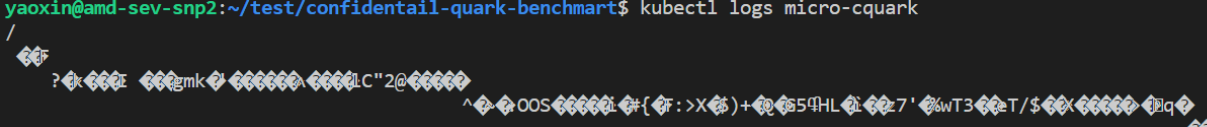
\includegraphics[clip,width=\columnwidth]{images/cquark_log_from_kubectl.png}%
    }
    
    \caption[Accessing application log through kubectl and securectl in confidential quark]{Accessing application log through kubectl and securectl in confidential quark. Figures 1 and 2 show that privileged users in cquark, i.e., 
    application owners, have normal access to the application logs, while non\-privileged users using kubectl logs only obtain encrypted garbled code.}
\end{figure}

\subsection{Storing Qkernel Log on host in plaintext}
In Vanilla Quark, guest kernel log messages are saved in the /var/log/quark directory on the host.  This arrangement could result in an untrusted entity like k8s operator, who has the access to the host,  obtain sensitive information from the logs(refer to Figure ~\ref{fig:vanilla_qkernel_Log}).
\begin{figure}[H]
    \centering
    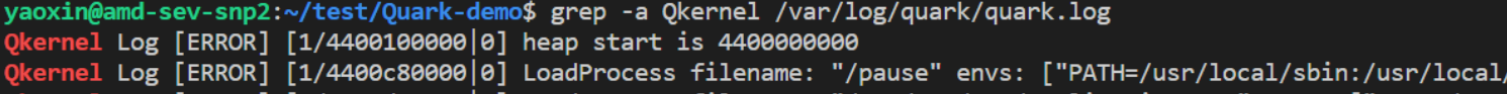
\includegraphics[width=1\textwidth]{images/vanilla_qkernel_Log.png}
    \caption[Accessing guest kernel log in vanilla quark]{Accessing guest log in vanilla quark. Note that both qvsivor and qkernel generate logs that are saved in the same file, i.e., /var/log/quark/quark.log. To distinguish between the logs, the logs generated by qkernel are prefixed with the keyword "Qkernel."}
    \label{fig:vanilla_qkernel_Log}
\end{figure}


To mitigate the security risk, confidential quark enables the application owner to specify the logging level of the guest kernel logging system in the shield policy. Presently, this logging system supports five log levels, ranging from Off (least detailed) to Trace (most detailed). The logging system only prints 
logs at a level equal to or below the level specified in the shield policy to host.  Currently, the log level in the enclave policy is configured to Off. As a result, guest kernel logging system will not print any logs to host (as illustrated in Figure ~\ref{fig:cquark_qkernel_log}).
\begin{figure}[H]
    \centering
    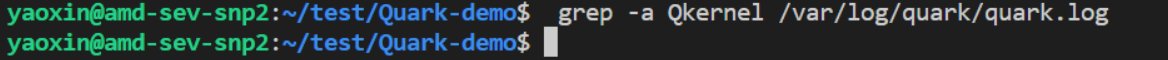
\includegraphics[width=1\textwidth]{images/cquark_qkernel_log.png}
    \caption[Accessing guest kernel log in confidential quark]{Accessing guest kernel log in confidential quark.  Note that both qvsivor and qkernel generate logs that are saved in the same file, i.e., /var/log/quark/quark.log. To distinguish between the logs, the logs generated by qkernel are prefixed with the keyword "Qkernel."
    Here we launch an application in cquark and try to access the qkerel logs under /var/log/quark directory. Since the log level in the policy file is set to Off, we can't get any qkernel log there}
    \label{fig:cquark_qkernel_log}
\end{figure}

\subsection{No restriction to application's syscalls (guest system call)}
Vanilla Quark does not provide any functionality to restrict the available system calls for an application. Consequently, an attacker can trick an application into executing a vulnerable system call to snoop on the application's confidential data. To address this issue,  confidential quark introduces a guest 
system call interceptor, which enables application owner to restrict the guest system calls that an application can invoke through the shield policy in Figure ~\ref{fig:generic_policy}.

\begin{figure}[H]
    \centering
    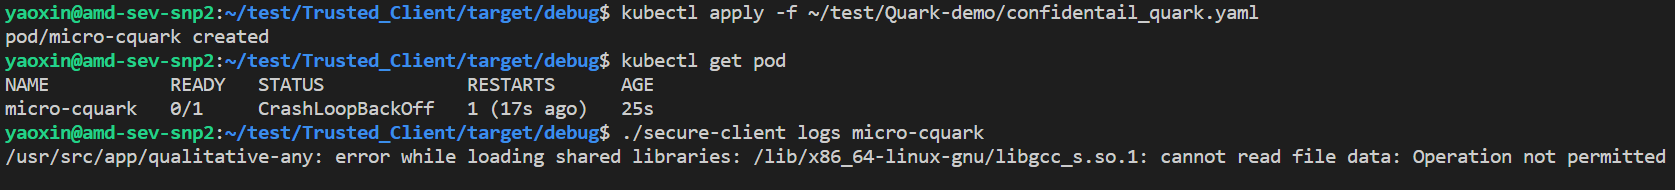
\includegraphics[width=1\textwidth]{images/application_failed_to_start_due_to_syscall_interceptor.png}
    \caption[Application failed to run due to the lack of permission to execute the read system call for loading dynamic libraries]{Application failed to run due to the lack of permission to execute the read system call for loading dynamic libraries}
    \label{fig:application_failed_to_start_due_to_syscall_interceptor}
\end{figure}


Figure ~\ref{fig:application_failed_to_start_due_to_syscall_interceptor} presents a demo of the guest interceptor. By revising the setting of the system interceptor in the enclave policy of Figure ~\ref{fig:generic_policy} to remove the read system call from the system call whitelist, 
the application process failed to start. The failure occurred because it lacked the permission to execute the read system call for loading dynamic libraries.
\subsection{Lack of runtime measurements}

The application binary and it’s runtime libraries in Vanilla Quark are stored on the host machine. The code is loaded into the guest memory only at runtime, which creates a potential vulnerability that an attacker may exploit to force the 
application to execute corrupted code, thereby compromising confidential information. In response, Confidential Quark provides two types of security measures:

\subsubsection{Application launch measurement}
During program startup (from the enclave starts until the application runs), the enclave measures the data it loads from the host, including the guest kernel configuration, the application process spec, and the application binary. The result 
of these measurements is known as the application launch hash, which is included in the remote attestation report sent to KBS. KBS subsequently compares the hash value to the reference hash value in the enclave policy, which was previously uploaded 
by the application owner. If the hash values do not coincide, KBS denies the transfer of any sensitive information to the enclave.
\begin{figure}[H]

    \subfloat[Application launch process and it's result\label{fig:cquark_launch_measurement_demo}]{%
      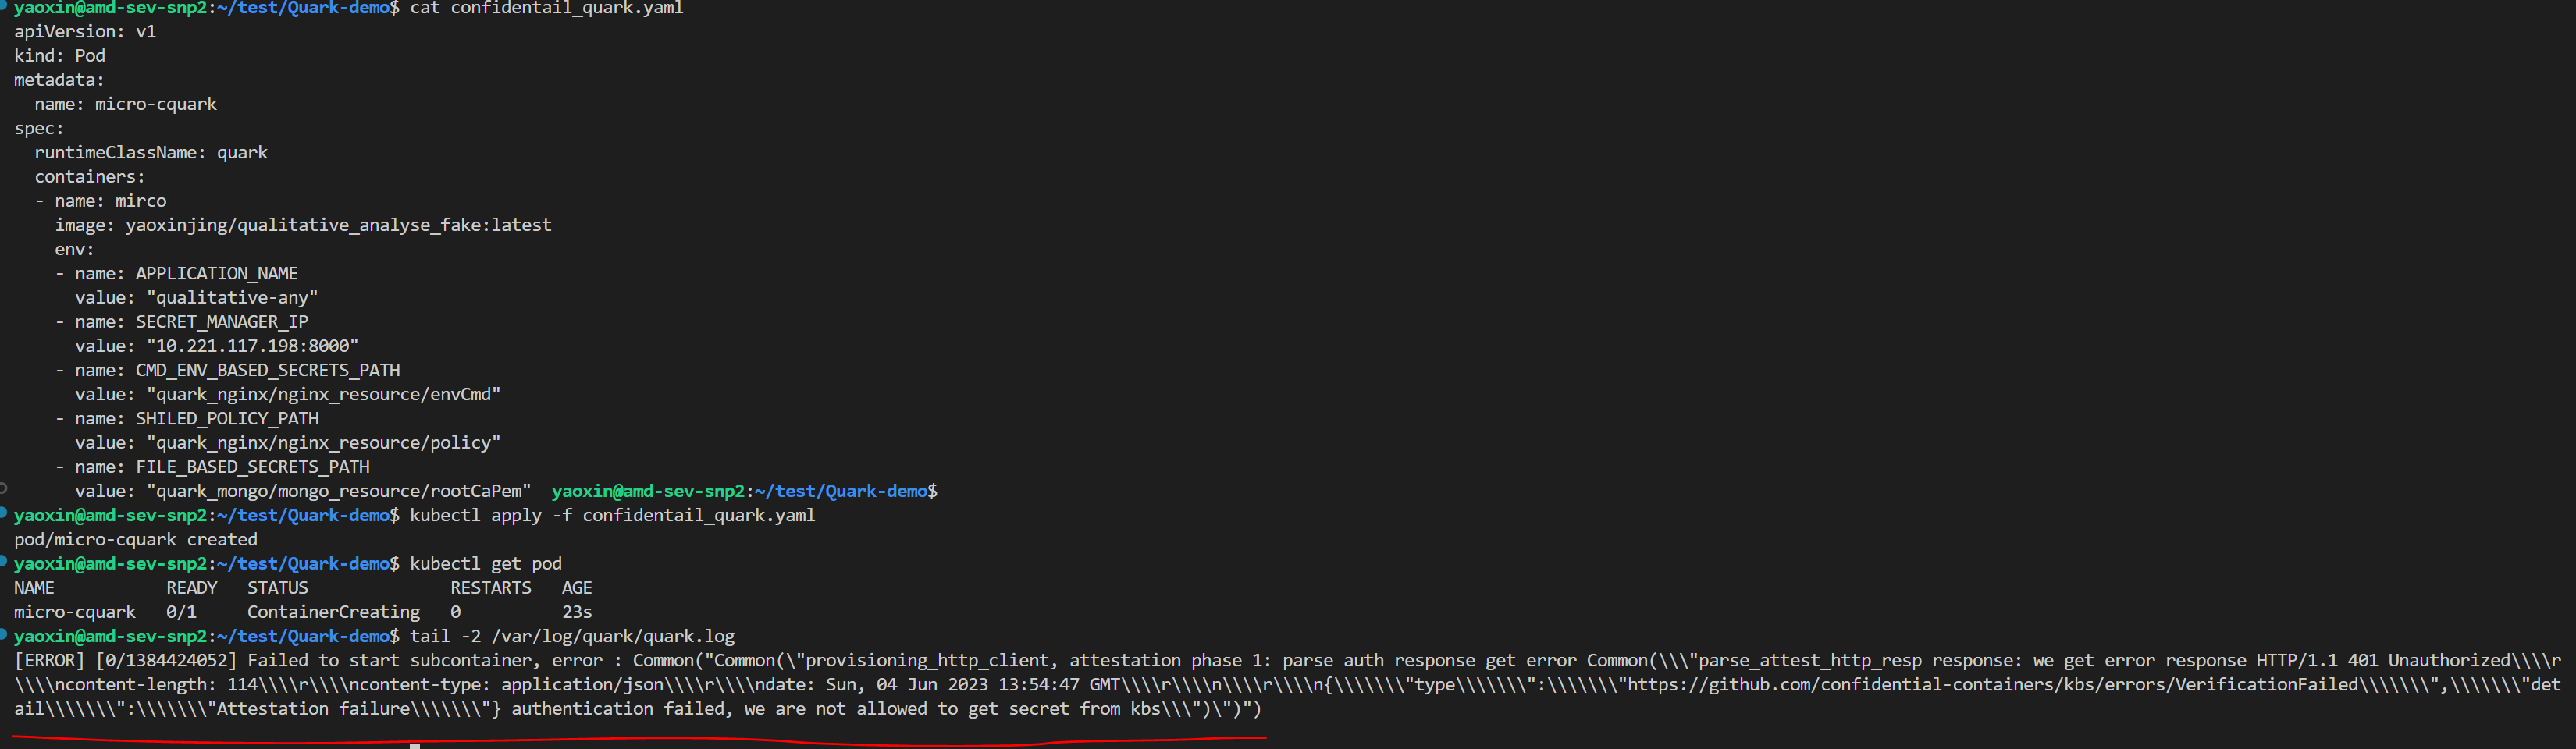
\includegraphics[clip,width=\columnwidth]{images/cquark_launch_measurement_demo.png}%
    }
    
    \subfloat[KBS rejected the enclave's authentication request due to a mismatch in application launch measurements\label{fig:cquark_launch_measurement_demo_kbs}]{%
      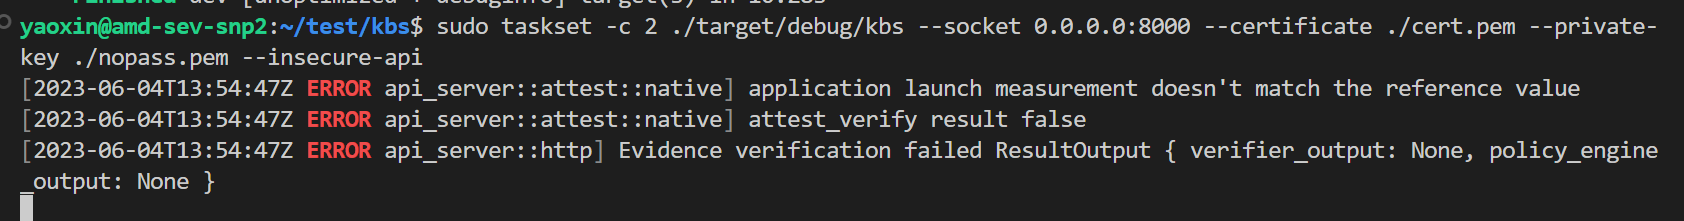
\includegraphics[clip,width=\columnwidth]{images/cquark_launch_measurement_demo_kbs.png}%
    }
    
    \caption[Application launch measurement demo]{Application launch measurement}
    \label{fig:cquark_launch_measurement}
\end{figure}

A demonstration is shown in Figure ~\ref{fig:cquark_launch_measurement}. Regarding the setup, we modifie the program\cite*{qualitativ_workload} in Figure ~\ref{fig:analysis_workload} (correspondent to image qualitative\-analyze) and create a new image labeled qualitative\-analyze\-fake. 
The altered image is then deployed to the micro\-cquark pod in an attempt to obtain the image "qualitative\-analyze" 's secrets. However, as shown in Figure ~\ref{fig:cquark_launch_measurement_demo_kbs}, KBS rejecte the request initiated by micro-cquark due to a mismatch between the 
application startup hash from the micro\-cquark pod and the reference application launch hash generated by qualitative-analyze image. In essence, the modification of the program caused the binary contents to change, resulting in startup measurements of the application launched from the 
 qualitative\-analyze\-fake image that does not correspond with the startup reference hash (for the original program) depicted in the enclave policy (Figure ~\ref{fig:generic_policy}). This experiment confirmed KBS would reject enclave requests if there is any modification 
 of data loading during the application startup process.


\subsubsection{Shared library/executable measurement at runtime}
Regarding runtime libraries and binaries loaded during application runtime, the enclave  measure the loaded data and compare the hash with the  reference hash in the enclave policy.

\begin{figure}[H]
    \centering
    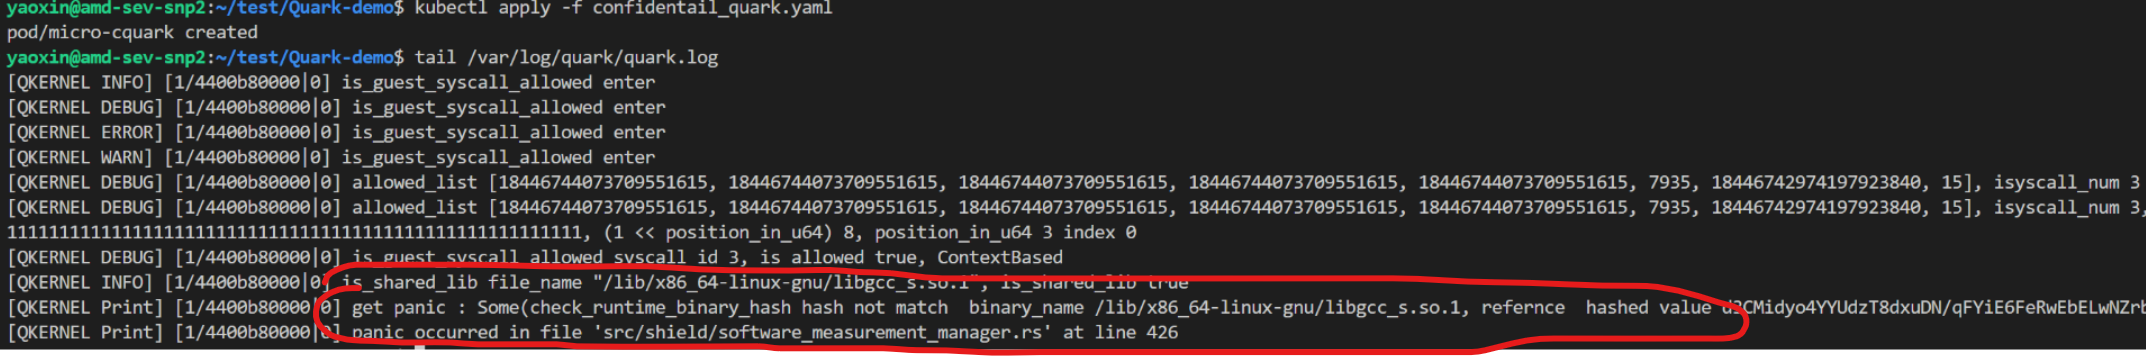
\includegraphics[width=1\textwidth]{images/cquark_runtime_runtime_lib_measurement_demo.png}
    \caption[Shared library measurement demo]{Shared library measurement demo}
    \label{fig:cquark_runtime_runtime_lib_measurement_demo}
\end{figure}

Figure ~\ref{fig:cquark_runtime_runtime_lib_measurement_demo} shows a demo of measuring the runtime library. As part of the setup, We reset the reference hash of  library "/lib/x86\_64-linux-gnu/libgcc\_s.so.1" in the enclave policy to empty and 
configure the logging level of Qkernel in the enclave policy to Info(refer to Figure ~\ref{fig:generic_policy}). Next, we deployed the program using the YAML in Figure ~\ref{fig:cquark_deployment} and observe the qkernel logs  The log reveales that the enclave encountered 
a crash due to a difference between the measurement of the loaded library and the corresponding reference hash stored in the policy. This finding highlights the enclave's ability to reject execution when an adversary seeks to deceive the enclave 
into loading harmful library code.

 \begin{figure}[H]
    \centering
    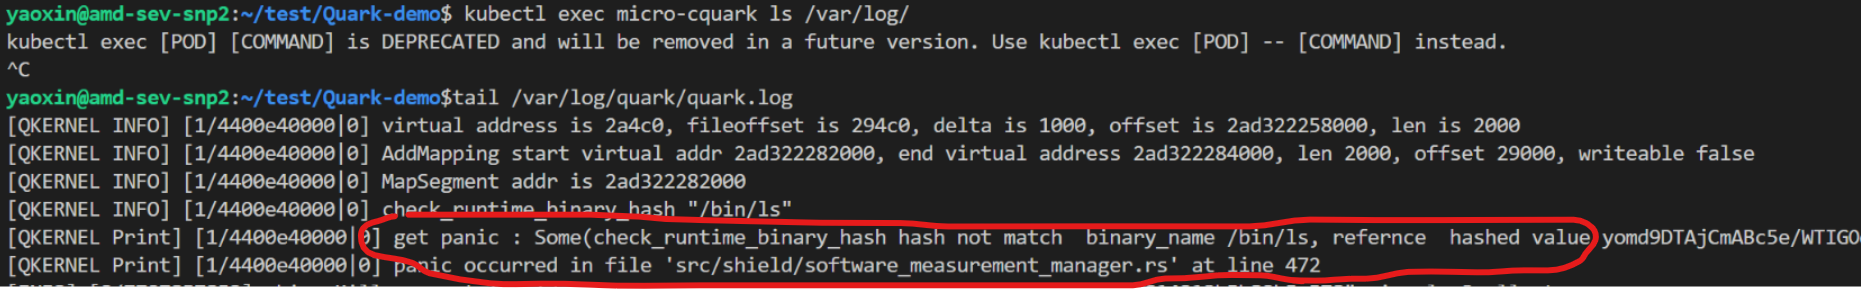
\includegraphics[width=1\textwidth]{images/cquark_runtime_runtime_binary_measurement_demo.png}
    \caption[Runtime binary measurement demo]{Runtime binary measurement demo}
    \label{fig:cquark_runtime_runtime_binary_measurement_demo}
\end{figure}


Figure ~\ref{fig:cquark_runtime_runtime_binary_measurement_demo} is a demo of measuring binary loaded at application runtime  As part of the setup, We reset the reference hash of ls binary in the enclave policy to empty and configure the logging level of Qkernel in the enclave policy to 
Info(Figure ~\ref{fig:generic_policy}). Subsequently, we facilitated deployment of the program using the YAML file in Figure ~\ref{fig:cquark_deployment} and executed the 'ls' command via 'kubeclt exec'\cite*{kubectl}, causing the enclave to load the 
corresponding 'ls'binary from the host. However, the command failed to elicit a response. Upon analysis of the Qkernel log, we confirmed that the Qkernel crashed due to a mismatch between the reference hash of  binary and its actual hash. 
This finding highlights the enclave's ability to refuse execution when an adversary attempts to trick the enclave into loading harmful binary code during application runtime.

\subsection{Missing administration to application restartup}

\begin{figure}[H]
    \centering
    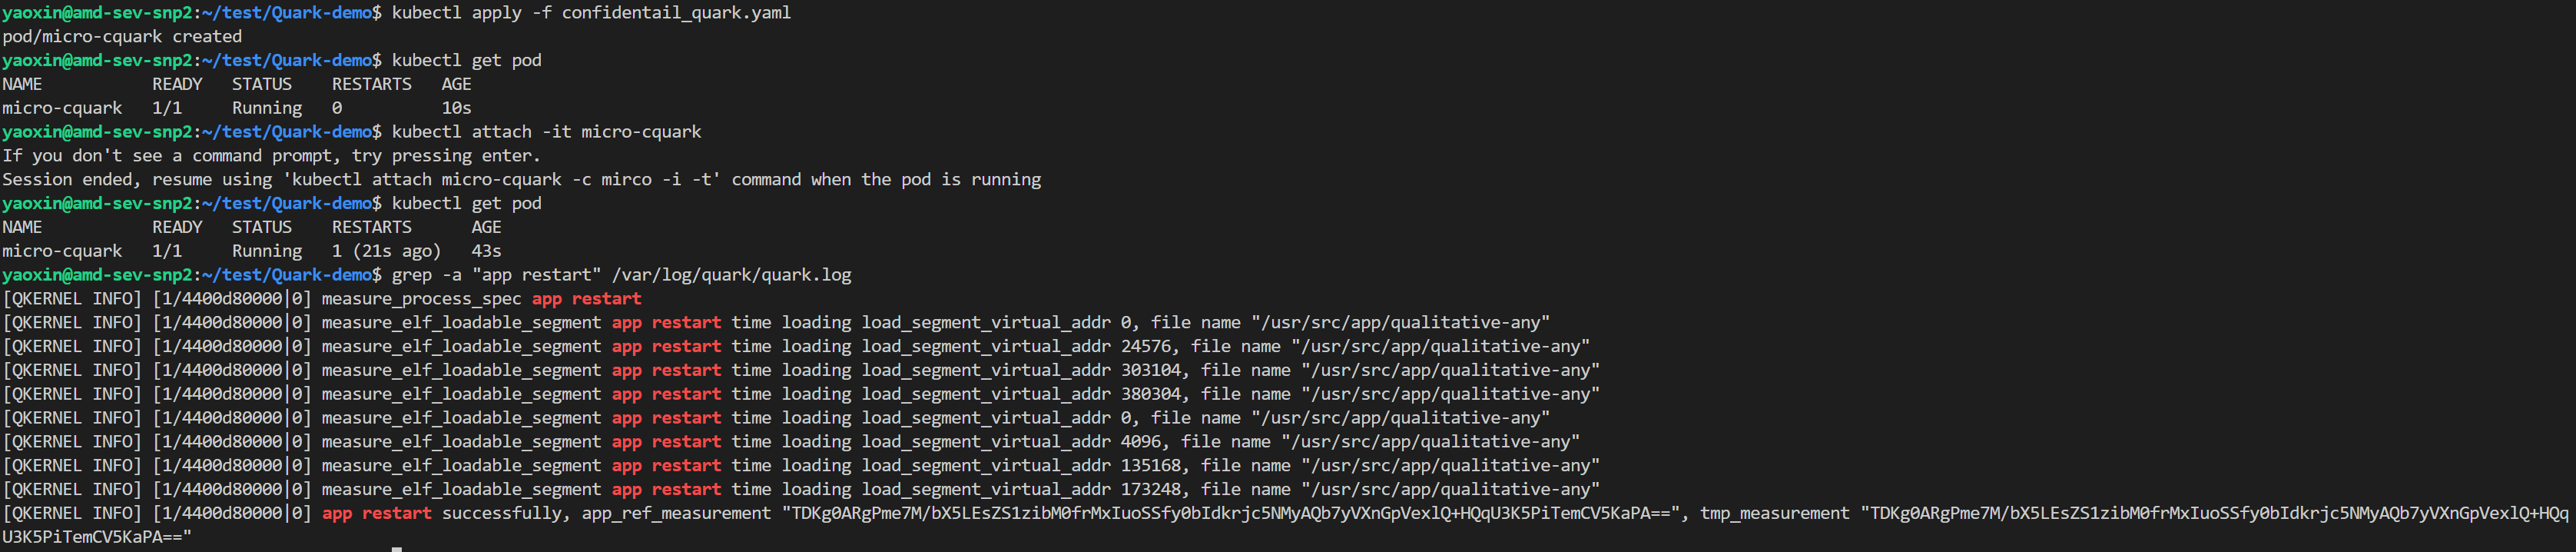
\includegraphics[width=1\textwidth]{images/cquark_restart_administration_demo.png}
    \caption[Demo for  administration to application restartup]{Demo for  administration to application restartup}
    \label{fig:cquark_restart_administration_demo}
\end{figure}



In the event of an unexpected application process exit, Kubernetes may elect to recreate a pod to run the crashed program, or restart the program within the original pod if it still exists\cite*{k8s}. In the latter scenario, the Qkernel must reload the application 
binary from the host, as well as the application process specification. Given that the application secrets are already stored within the enclave, remote attestation is skiped during application restart , meaning that the relying party is unable 
to verify the integrity of the host loaded data. This opens the possibility for an attacker to provide the enclave with corrupted code. To address this risk, Enclave in confidential quark stores the hash value of the initial application 
startup, known as app\_ref\_measurement, on guest memory. During the application rebuild process, cquark measures host-loaded data and calculate the hash value known as tmp\_measurement.  Enclave will compare these two hash values to ensure that the re-creation 
process is correct.

The processes described above are exemplified in Figure ~\ref{fig:cquark_restart_administration_demo}. In this example, we configure the Qkernel log level to 'Info' in the enclave policy displayed in Figure \ref{fig:generic_policy}, and add the keywords 
'stdin: true' and 'tty: true' to the container spec of the YAML file used to deploy the application (as shown in Figure ~\ref{fig:cquark_deployment}). These keywords keep the application's stdin open and signal to Kubernetes that it should 
be regarded as a terminal. In the demo, we first create the application using the modified YAML file. Once the application started, we use 'kubectl attach -it' to establish a connection with the application's stdin and halted the program using 'ctrl c'. The output of the second 'kubectl get' 
command in Figure ~\ref{fig:cquark_restart_administration_demo} confirmed that the program had succesfully restarted. After analyzing the Qkernel log, we find that Qkernel measured the process spec and application binary loaded from the host during application recreation. This measurement is saved in the 
'tmp\_measurement' variable and compared to the hash value, 'app\_ref\_measurement' before the program process entered the user space.




\subsection{Vulnerability Out of Scope}
Besides the vulnerabilities already discussed, there are other security risks that affect Vanilla Quark but are beyond the scope of this thesis.



\textbf{Physical Access Attacks.} An untrustworthy entity, including cloud operators who have physical access to the machine where the application runs, can carry out physical access attacks on the system. One example of such attacks 
is Offline DRAM Analysis. A partial solution to alleviate the threat is to run guest on AMD SEV SNP or INTEL TDX.  Those interested in learning more about this topic should refer to \cite*{SEV_SNP_white_book}, \cite*{DBLP:journals/corr/abs-2303-15540}.


\textbf{Lack of protection to guest memory and register states.} Lack of protection to guest memory and register states.  Insufficient protection for guest memory and register states allows non-trusted entities, such as a hypervisor, to access guest confidential, leading to security breaches. 
Trusted execution hardware like AMD SEV\cite*{SEV_SNP_white_book} and Intel TDX\cite*{Intel_tdx_whitepaper} address this by encrypting guset memory and registers. However, CQuark does not yet support running on the Trusted execution hardware yet.


\textbf{Paravirtualized filesystem sharing mechanism.} Vanilla Quark uses this mechanism to share files and volumes stored on the host with applications on the guest. Any modifications made by an application on a file will be reflected on the host. This poses a security risk as an attacker could 
gain access to application’s confidential by accessing the application's rootfs on the host. To address this, a common approach is to implement a guest filesystem shielding layer to cryptographically protect inbound and outbound guest data. Those interested in learning more about this topic should 
refer to \cite*{file_system_shield}.


\textbf{No security guarantee for communications over the Internet (unbounded network access to containers).} The qkernel in Vanilla Quark lacks authentication to network requests and cryptographic protection for transmitted data, resulting in potential unauthorized access to the application or 
man-in-the-middle attack\cite*{Man_in_the_middle_attack}. For instance, attackers can use Kubectl port forwarding to connect to an application listening on the target port and acquire the application’s confidential data or service. A possible solution to this is implementing a guest network shield that leverages TLS to authorize 
incoming network requests and provides cryptographic protection for incoming and outgoing data. However, this thesis does not cover this type of vulnerability, and readers are encouraged to refer to reference \cite*{network_shiled}.

\textbf{Side channel attack.} Side channels, such as TLB side channel\cite*{217454}, cache side channel\cite*{7163050}, ciphertext side channel\cite*{274707} , and page-fault side-channel\cite*{236278}, can jeopardize the confidentiality of programs.  This type of vulnerability is considered out of the scope.



% \begin{table}[H]
%     \tiny
%     \caption{Possible Vulnerability in upstream Quark in the context of Confidential Computing and suggested Solutions}
%     \label{crouch}
%     \begin{tabular}{  p{3.4cm}  p{3.4cm}  p{3.4cm} p{2cm} }
%         \toprule
% \textbf{Vulnerability}      
% & \textbf{Attack Example}   
% & \textbf{Possible Solution}
% & \textbf{Comment}  \\\midrule
% Physical Access Attacks
% & Offline DRAM Analysis          
% & Running the application in a secure virtual machine
% & Out of the scope   \\\hline
% Lack of protection to guest memory and register states          
% & Hypervisor reads private guest memory/cpu states                          
% & Running the application in a secure virtual machine
% & Out of the scope   \\\hline
% Paravirtualized filesystem sharing mechanism       
% & Hypervisor/Untrusted host process reads application’s credentials stored on host
% & Enable file system shielding layer to encrypt outbound and decrypt inbound data 
% & Out of the scope   \\\hline

% No security guarantee for communications over the Internet (unbounded network access to containers)     
% & Attacker access application’s credential by establishing a network connection to application using tools like, kubectl port-forward
% & Enable network shielding layer using TLS
% & Out of the scope   \\\hline

% Deploying Secrets via untrusted Entities (Kubelet, Containerd, Qvisor)    
% & File type secrets are mounted to container rootfs by qvisor, args and envv type secrets are passed to qkernel through qvisor
% & Offload the secrets deployment from qvisor by defining a new secure channel btw. relying party and guest kernel for secrets provisioning and storing secrets on guest memory
% & Problem solved  \\\hline

% Executing arbitrary command in container  
% & Attacker view application’s credentials stored on guest memory using kubectl exec cat command
% & Enable authentication and access control to kubectl exec in guest kernel
% & Problem solved  \\\hline


% Container log in plaintext managed by untrusted entity
% & Attacker reads application’s log message using kubectl logs container-name
% & Enable container STDOUT protection
% & Problem solved  \\\hline

% Storing Qkernel Log on host in plaintext
% & Cloud provider reads guest kernel’s log messages located in directory /var/log/quark
% & Enable qkernel log manager and set the log level to OFF
% & Problem solved  \\\hline

% Loading untrusted executable from host
% & Attackers may tamper with executables stored on the host and trick applications into executing compromised code to reveal secrets
% & Executable loaded into guest memory is measured and the results are send to relying party for executable integrity check
% & Problem solved  \\\hline

% Loading untrusted shared library from host
% & Attackers may tamper with shared libraries stored on the host and trick applications into executing compromised code to reveal secrets
% & Executable loaded into guest memory is measured and the results are send to relying party for executable integrity check
% & Problem solved  \\\hline

% Missing administration to application restart
% & Attacker may provide the guest with compromised executables, shared libraries, or wrong process spec when k8s requests the Qkernel to restart the crashed application
% & Compare the hash of the application rebuilding process with the hash of application's initial launching process stored on guest memory. If two hashes doesn’t match,  qkernel refuse the application restart request.
% & Problem solved  \\\hline


% No restriction to Container's syscalls (guest system calls)
% & Applications can be tricked into using vulnerable guest/host system calls, leading to disclosure of secrets
% & Using Guest system call interceptor to restrict the system calls application can use.
% & Problem solved  \\\hline


% Creating application process using untrusted process spec sent from host
% & Attacker may trick the qkernel into attaching a terminal to application process by modifying the "terminal" option in the process specification
% & Software measurement manager measure the loaded process specification and the results are send to relying party for integrity check
% & Problem solved  \\\hline


% Lack of runtime measurements
% & Secure VM like AMD SEV only calculate the hash of VM launching process, anything loaded to guest during runtime is not measured
% & Add software measurement manager to measure data loaded during runtime
% & Problem solved  \\\hline
% % objects and systems &
% % Underlying values       
% % & Plurality \\
%         \bottomrule
%     \end{tabular}
% \end{table}


\section{Quantitative Analysis}
In this section, we evaluate the performance of the system implementations described in the previous chapters through multiple benchmarks to assess the impact on the throughput and latency of the applications running in the confidential quark environment.


\subsection{Overview of Quantitative Analysis}

Our benchmarks  consist of micro-benchmarks and macro-benchmarks. The microbenchmarks are performed to  thoroughly understand the latency overhead of each new building block in CQuark, while the macro benchmarks are conducted to compare the speed of 
real world applications run by confidential vs vanilla Quark. This give us a view of the overhead incurred by confidential Quark for protecting application’s confidentiality.


The benchmarking in this section is structured around the following subsections. First, we describe the hardware and software setup for benchmarking in Section \ref{Hardware_and_Software_Setup}. We then evaluate the speed of obtaining three different types of attestation reports (emulated hardware 
reports, software reports signed by the kbs key or by the application key) using a microbenchmark that executes a certain number of a system call in a loop and records the time required to execute the system call (Section \ref{Attestation_Report_Syscall}). We found that the speed of obtaining the 
emulated hardware report is 50\% slow than that of obtaining the other two reports due to VM exit. 

Subsequently, in Section \ref{bench_Interceptor}, we evaluate the overhead of the guest system call interceptor using a micro test that executes a certain number of a specific system call in a loop in vanilla and confidential Quark, respectively. The results show that the guest system interceptor imposes an overhead of 1.47x 
and 17x for system calls that are handled only by the guest and system calls that must be handled by the host, respectively

Unlike vanilla Quark, which stores file-type secrets on the host, cquark stores file-type secrets directly on guest memory. Therefore, in Section \ref{bench_reading_file_secret}, we evaluate the speeds of an application accessing file-type secrets in vanilla and confidential Quark using a similar 
approach as in Section \ref{Attestation_Report_Syscall}. The results reveal that in confidential Quark, the speed of accessing file-type secrets is improved by a factor of 1.17.

% the authentication and access control for the exec endpointin 
Later, in Section \ref{bench_issuing_Instructions}, we present latency  benchmark results for sending commands to containers in confidential and vanilla Quark. Compared to the speed of sending commands using kubectl exec\cite*{kubectl} in vanilla quark, confidential Quark's implementation 
introduces 1.15 times overhead. Furthermore, We compare the speed of sending the same command with kubectl and securectl in confidential Quark. The results show that despite the additional encryption and decryption required by the commands sent by securectl, the commands are 
executed 1.1 times faster than those sent by kubectl.

Then after conducting an evaluation of the performance of accessing binary-mapped memory regions in cquark, we observed that confidential quark outperforms vanilla quark in this regard (Section \ref{accesiing_binary_mapped_memory}). Sequential access in confidential quark is 1.86 times faster than in 
vanilla quark, while random reading and writing of binary-mapped memory regions exhibit approximately 1.08 times faster speed in confidential quark. These results can be attributed to confidential quark's measurement of binary files during program startup, which prompts the qkernel to load 
the files into memory, thus preventing  page fault handling during runtime.

In Section \ref{micro_app_start_up}, we conducted an evaluation of the latency overhead introduced by the our implementation during application deployment using a "hello world" program.  Specifically, the evaluation involved testing the latency overhead of the attestation and provisioning agent, 
secret injector, software measurement manager, and hardware evidence driver. Throughout the experiments, we adjusted a critical parameter to observe how each component affects the overall application startup time. Findings indicate that the attestation and provisioning agent constitutes 
the bulk of the overhead when the size of the measurement data is less than 100 MB, while the overhead introduced by the secret injector and hardware evidence driver is negligible in any case. 
% Further details, including the benchmark configuration and results can be found on page XX.

In Section \ref{macri_app_start_up}, we conclude the performance benchmarking exercise by conducting macro benchmarking using Nginx \cite*{nginx} and Redis \cite*{redis} as workloads. Our benchmarks focus on exploring the performance differences between applications running in confidential and vanilla Quark 
in terms of startup time, exit time, and the application throughput. Our findings reveal that in confidential Quark, Redis \cite*{redis} and Nginx \cite*{nginx} require 1.49X and 1.55X startup times than in vanilla quark, respectively. The difference of startup time between Nginx and Redis in 
confidential Quark primarily arises from the contrast in data size measured during application startup, i.e., 67.15 Mib in Nginx and 16.258 MiB in Redis. In terms of application exit time, Redis and Nginx exhibit nearly identical performance when running on confidential  and vanilla quark. 
Furthermore, we utilized Redis-benchmark \cite*{Redis_benchmark} and Apache HTTP server benchmarking tool \cite*{ab} as load generators to gauge the application's throughput. Our experiment results indicate that Nginx and Redis running in cquark encounter performance declines of approximately 
9\% and 20\%,respectively, due to guest system interceptor.

In Section \ref{tcb}, we evaluated the TCB overhead incurred by our implementation and compared the TCB size of the Confidential Container \cite*{confidential_kata} with that of the confidential Quark. Our findings reveal that our implementation increases the quark guest kernel binariy by approximately 1.47 times. Nevertheless, 
the TCB of confidential Quark is only roughly one-sixteenth of the size of the  Confidential Container \cite*{confidential_kata}.

\subsection{Hardware and Software Setup}\label{Hardware_and_Software_Setup}

In this section, a summary of the hardware and software settings utilized for the benchmarks is provided. Regarding hardware, all measurements are performed on a server with AMD EPYC 7443P 24-Core cpu and 4 DDR4-3200 Mhz-16GB RAM. In terms of software, the host OS is Ubuntu 20.04.6 LTS and Linux 
5.19.0 kernel. To establish a low-noise environment for benchmarking with reproducible results, the CPU governor is set to performance mode, and Hyper-Threading and Turbo Boost were disabled.  Moreover, all binaries used for testing, namely Qvisor, Qkernel, and the "hello-world" program in List ~\ref{code1}, 
are built in release mode. Note that, unless otherwise mentioned, the vanilla Quark is in version v0.2.0, confidential Quarkuses this commit  \cite*{qualitativ_confidentail_quark} in the following.


Regarding the tools for measuring latency, since all benchmark objects are located in the guest, we use the guest system call clock\_gettime(monotonic) \cite*{clock_gettime} for time measurement and print the results to the host using the qkernel logging system. The benchmarking framework \cite*{benchamark_framework} can analyze the 
results by parsing the confidential quark log located under host directory /var/log/quark.

In addition, all benchmarks are performed multiple times to minimize the impact of environmental noise on the results. Figures in the following sections illustrate the measurement results, conveying the average time and variance utilized for one run of the subject being measured.

\subsection{Micro-benchmark – Attestation Report Syscall}\label{Attestation_Report_Syscall}

Confidential quark enables guest user mode applications to obtain three types of attestation reports, that is, simulated AMD SEV SNP reports, software reports signed by KBS keys, or software reports signed by the application via a system call. In this section, we assess 
the speed with which the application acquires various attestation reports.

\begin{figure}[H]
    \centering
    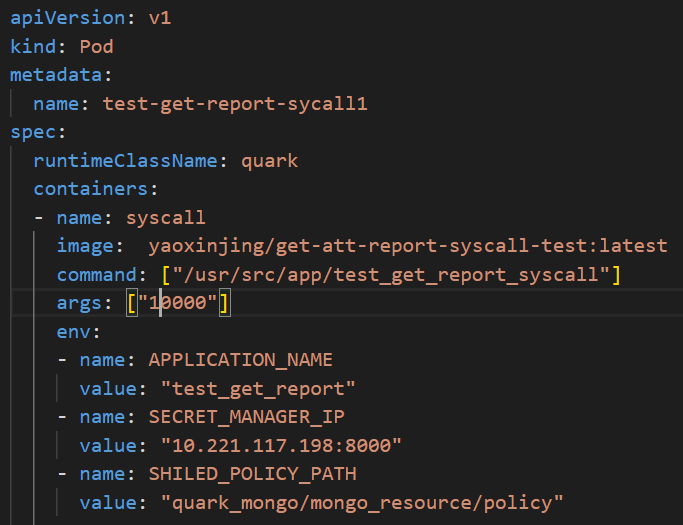
\includegraphics[width=0.8\textwidth]{images/perf_attestation_report_yaml.PNG}
    \caption[Qkernel Attestation Report Syscall Benchmark Deployment]{Qkernel Attestation Report Syscall Benchmark Deployment}
    \label{fig:perf_attestation_report_yaml}
\end{figure}

To this end, we prepared a Rust microbenchmark \cite*{benchamark_Attestation_Report_Syscall} that measures the mean and variance of the time requisite for obtaining the three types of reports and prints the results to its standard output. To ensure stable outcomes, the test program submits 10,000 requests for each type of report to the kernel. 
As the benchmark program is containerized, we can deploy the benchmark to Cquark using the YAML file in Figure ~\ref{fig:perf_attestation_report_yaml}.

\begin{figure}[H]
    \centering
    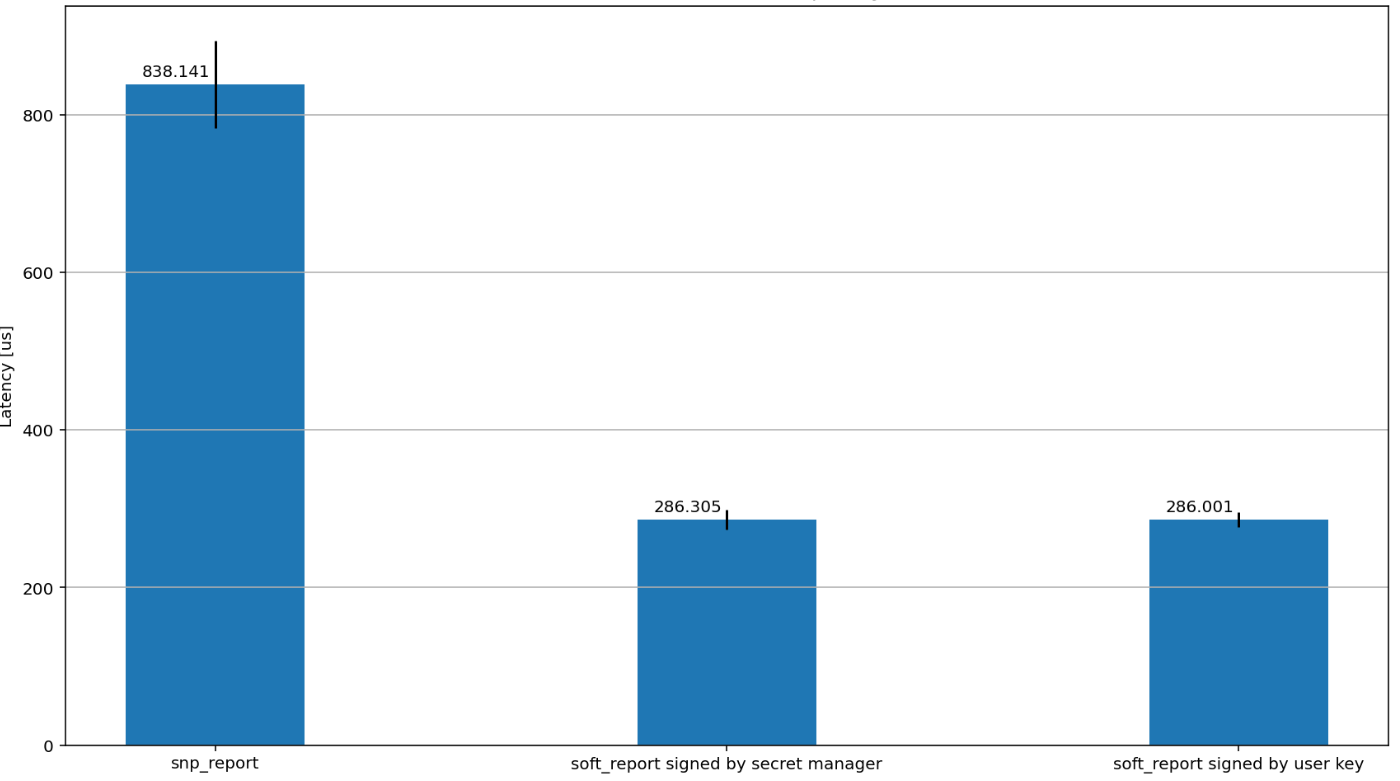
\includegraphics[width=0.8\textwidth]{images/perf_attestation_report_result.PNG}
    \caption[Benchmark result of Attestation Report Syscall]{Qkernel Attestation Report Syscall Benchmark Result}
    \label{fig:perf_attestation_report_result}
\end{figure}

Figure \ref{fig:perf_attestation_report_result} depicts the speed of requesting three types of attestation reports for  applications in the confidential Quark. The data reveal that acquiring a software report requires approximately one-third of the time needed to obtain a simulated hardware report. 
Specifically, requesting a simulated hardware report takes approximately 838.141us, whereas acquiring the two software reports needs only about 286us. The disparity stems from the dissimilarities in processing software and hardware reports by the qkernel. While the qkernel 
system call handler generates software reports promptly, the handler needs to transmits hardware report requests through qkernel snp attestation driver to the host AMD SEV emulation module in order to generate a dummy report. This process involves expensive operations like VM exit, 
encryption and decryption of messages for communication between the snp attestation driver and host AMD SEV emulation modul, reading the on-disk dummy snp report among others. Consequently, acquiring a simulated hardware repors is significantly slower than obtaining a software report.


\subsection{Micro-benchmark – Qkernel Syscall Interceptor}\label{bench_Interceptor}

Interception guest system calls introduces latency overhead to applications running in the confidential Quark.  To investigate this overhead, we employ a micro benchmark program written in Rust\cite*{benchamark_systemcall_intercetion}.  The benchmark measures the average and variance execution 
time of chosen system calls. Furthermore, to obtain stable results., each system call is executed in a loop of 100,000 times. As the benchmark program is containerized, we can deploy the program to Cquark and upstream Quark using the YAML file in Figure \ref{fig:syscall_interceptor_yaml}.
\begin{figure}[H]
    \centering
    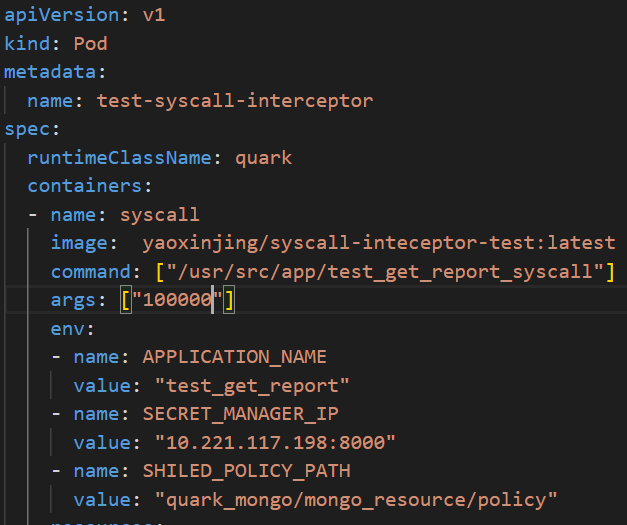
\includegraphics[width=0.8\textwidth]{images/perf_system_call_interceptor_yaml.PNG}
    \caption[Qkernel Syscall Interceptor Benchmark Deployment]{Qkernel Syscall Interceptor Benchmark Deployment}
    \label{fig:syscall_interceptor_yaml}
\end{figure}


For this benchmark, we select four system calls: getpid, getppid, read, and write. Since qkernel already implements process and thread objects, calling getpid or getppid using syscall instruction prompts qkernel to directly return the corresponding pid/ppid without interference from the host. 
This provides us with a clear understanding of the overhead introduced by the interceptor. Additionally, we measured the execution time of read and write system calls for confidential and vanilla Quark to evaluate the overhead that the interceptor brought to the host-handled system calls
\begin{figure}[H]
    \centering
    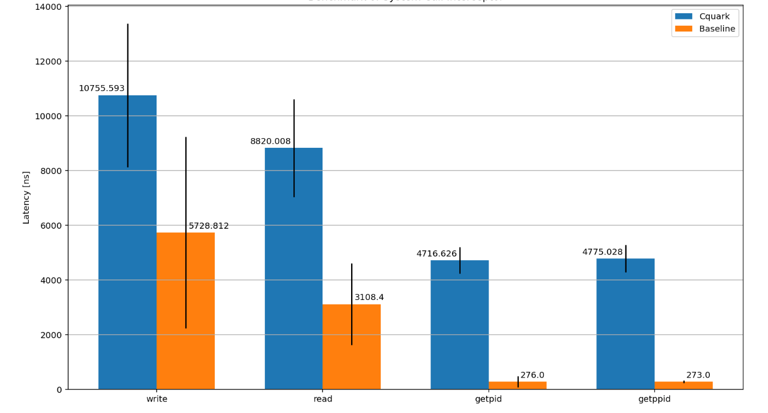
\includegraphics[width=0.8\textwidth]{images/ben_results_syscall_interceptor.PNG}
    \caption[Benchmark result of Syscall Interceptor]{Latency comparison of executing syctem calls in Cquark vs upstream Qaurk. The latency is thereby measured using the guest system call clock\_gettime(monotonic). 
        Each system call is executed 1,000,000 times in a tight loop. Read and write buffer size is 100 bytes}
    \label{fig:ben_results_syscall_interceptor}
\end{figure}


Figure ~\ref{fig:ben_results_syscall_interceptor} illustrates the mean and variance of execution times for the selected system calls in the both environments. We observed that vanilla Quark takes only around 270 ns to execute a single getpid and getppid call while confidential Quark
takes approximately 4716 ns. This implies that the guest system call interceptor causes a delay of about 4500 ns per system call. Moreover, a comparable latency overhead is introduced for read and write system calls, i.e.,4500 ns.  However, since read and write system calls are processed on 
the host side and take longer, their processing time in confidential Quark does not rise as significantly as that of getpid and getppid. To summarize, in confidential Quark, host handled system calls  (i.e., write and read) and guest handled-only (e.g., getpid and getppid) are 1.47x and 
17x slower, respectively, compared to vanilla Quark


The overhead incurred by the system call interceptor arises from two primary sources. Firstly, the whitelist of the guest system call interceptor is kept in a vector. Accessing the whitelist for system call authorization check is an operation with the complexity of O(N). 
Secondly, to avert any contentions resulting from run-time updates and reads to the system call interceptor's metadata, this metadata is safeguarded with a lock. Consequently, a lock/unlock operation is initiated for every system call permission check.



\subsection{Micro-benchmark – Speed of Reading file base secret}\label{bench_reading_file_secret}

Compared to vanilla Quark which stores file type secrets on the host, confidential Quark instead stores them on guest memory to prevent unauthorized access and avoid potential VM exits during read and write operations. Hence, the purpose of this benchmark is to evaluate the performance 
enhancement achieved from accessing file type secrets in confidential Quark. The benchmark\cite*{benchamark_filebase_secret} measures the total time taken to perform one open() and read() operation on a target secret type file in both environments. The file size is 1302 bytes. To ensure stable results, 10,000 open and 
read operations are performed. As the benchmark program is containerized, we deploy it to both confidential and vanilla Quark using the YAML file outlined in Figure ~\ref{fig:file_type_secret_access_test_deploy_yaml_baseline} and ~\ref{fig:file_type_secret_access_test_deploy_yaml_cquark}.


% \begin{figure}[H]
%     \centering
%     \subfloat[\centering Deployment File for upstream Quark]{{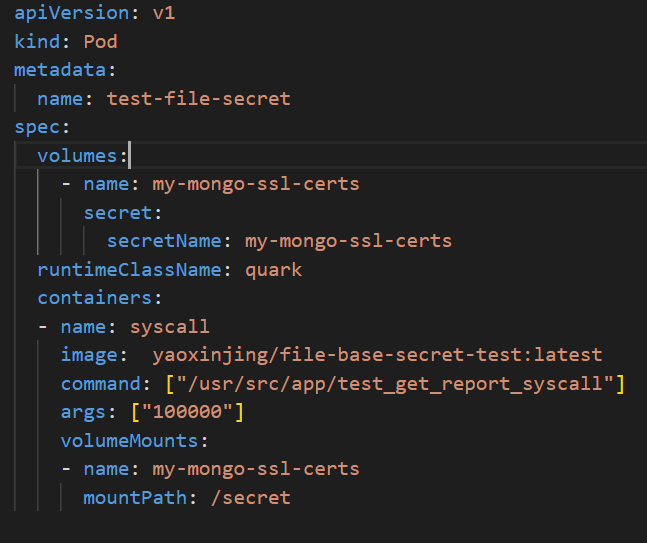
\includegraphics[width=5cm]{images/file_type_secret_access_test_deploy_yaml_baseline.PNG} }}
%     \qquad
%     \subfloat[\centering Deployment File for confidential Quark]{{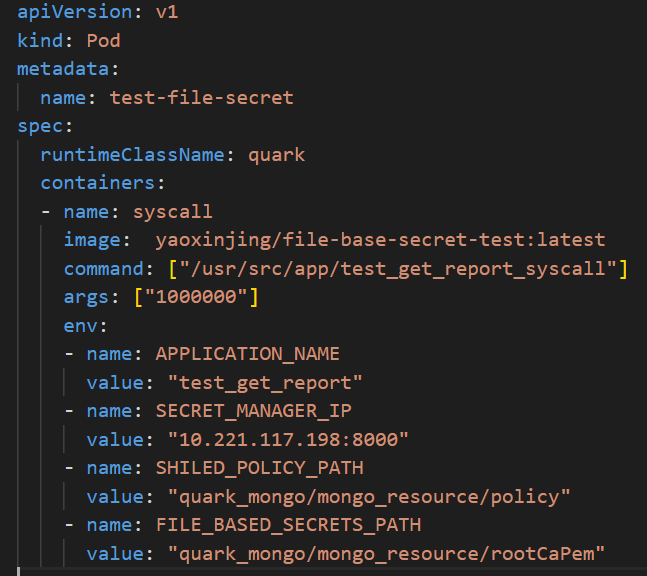
\includegraphics[width=5cm]{images/file_type_secret_access_test_deploy_yaml_cquark.PNG} }}
%     \caption{Benchmark Deployment for testing Speed of Reading file type Secrets }
%     \label{fig:file_type_secret_access_test_deploy_yaml_baseline}
% \end{figure}
% \end{document}

\begin{figure}
    \centering
    \begin{minipage}{0.45\textwidth}
        \centering
        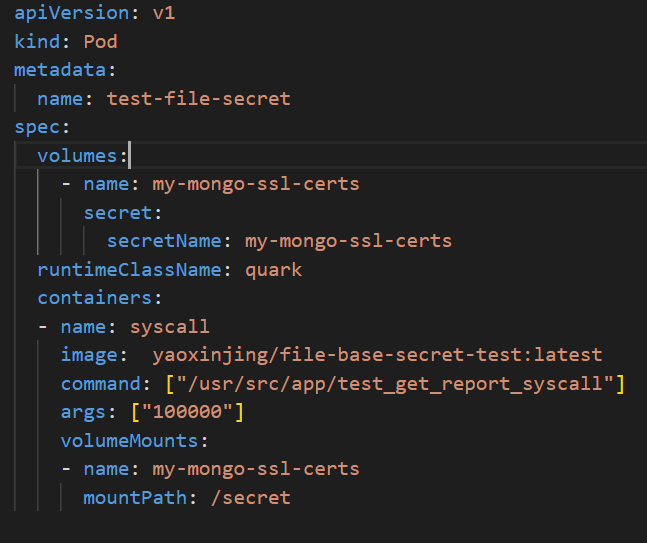
\includegraphics[width=0.9\textwidth]{images/file_type_secret_access_test_deploy_yaml_baseline.PNG} % first figure itself
        \caption{Benchmark Deployment for testing Speed of accessing file type Secrets in upstream Quark}
        \label{fig:file_type_secret_access_test_deploy_yaml_baseline}
    \end{minipage}\hfill
    \begin{minipage}{0.45\textwidth}
        \centering
        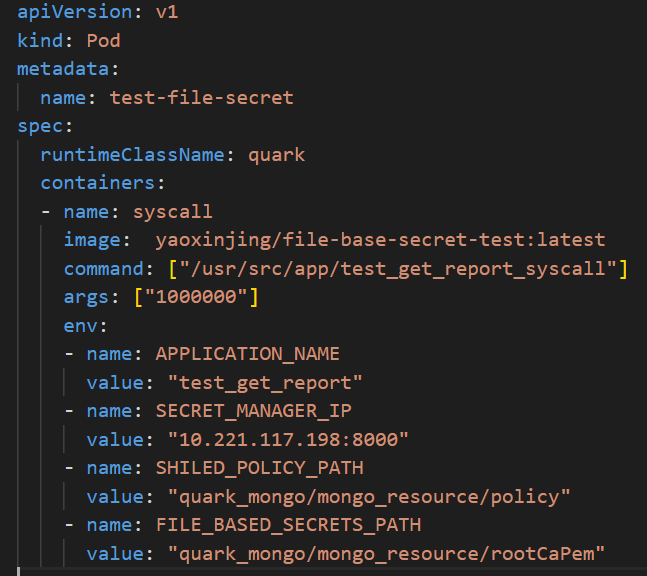
\includegraphics[width=0.9\textwidth]{images/file_type_secret_access_test_deploy_yaml_cquark.PNG} % second figure itself
        \caption{Benchmark Deployment for testing Speed of accessing file type Secrets in confidential Quark}
        \label{fig:file_type_secret_access_test_deploy_yaml_cquark}
    \end{minipage}
\end{figure}
\todo{update Benchmark Deployment for testing Speed of accessing file type Secrets in upstream Quark, change it to 100000}


\begin{figure}[H]
    \centering
    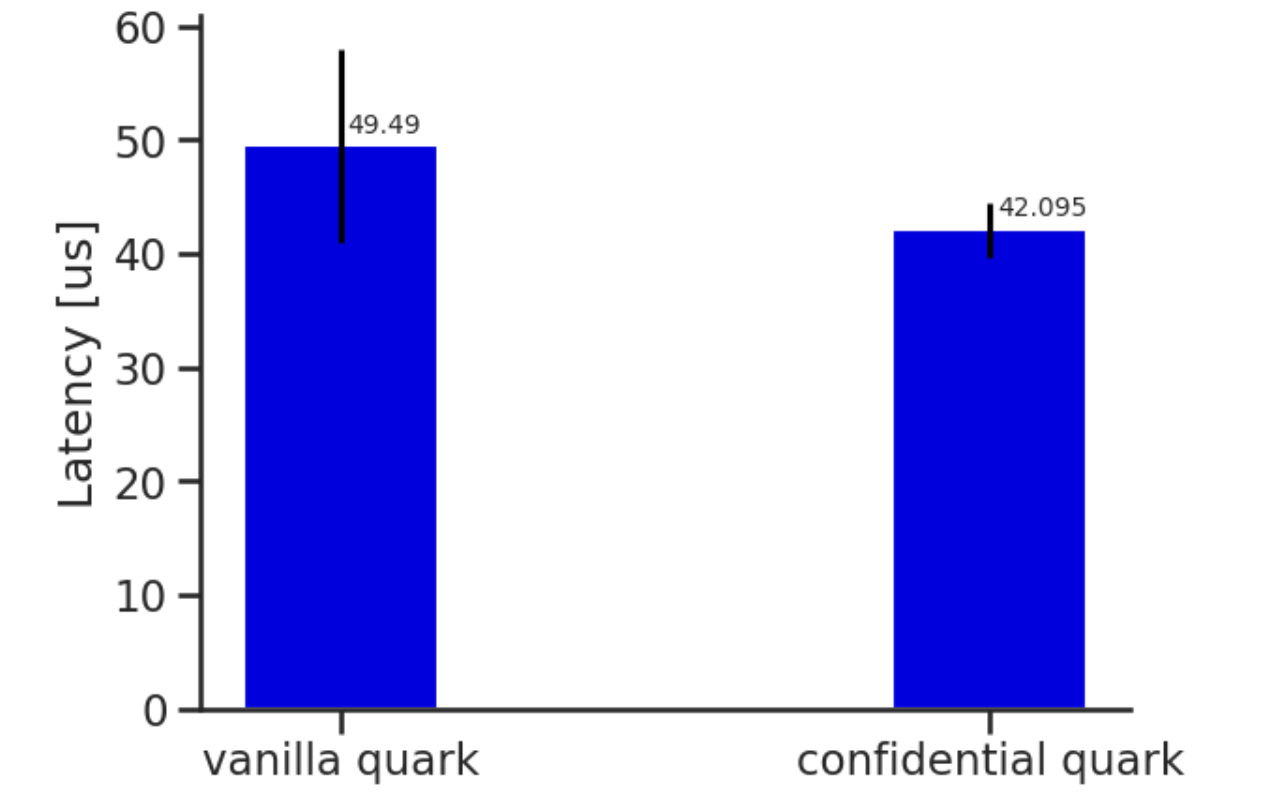
\includegraphics[width=0.8\textwidth]{images/reading_speed_of_file_type_secrets_in_Baseline_and_Cquark.PNG}
    \caption[Benchmark result of testing Speed of accessing file type Secrets in confidential Quark vs upstream quark]{The figure shows result of testing speed of accessing file type secrets in confidential vs vanilla Quark. 
    The evaluations is performed using the open() and read() system calls, and ten thousand (10,000) operations are conducted with a 50-byte read buffer size.
    }
    \label{fig:reading_speed_of_file_type_secrets_in_Baseline_and_Cquark}
\end{figure}


The obtained results are presented in Figure ~\ref{fig:reading_speed_of_file_type_secrets_in_Baseline_and_Cquark}, revealing that the performance  in confidential Quark is competitive with vanilla Quark for accessing file-type secrets. Surprisingly, there is no significant difference in speed
between the two, with confidential Quark providing only 1.17 times the performance improvement when accessing the target secret file.  The reason is that the larger performance loss resulting from system call execution due to the client system call interceptor in confidential Quark outweighs the overhead produced by VM exits in vanilla Quark.


\subsection{Micro-benchmark – Latency Test for issuing Instructions to Application}\label{bench_issuing_Instructions}

This section presents the results of tests conducted to assess the latency of issuing instructions to applications in confidential Quark. The tests involved comparing the latency of sending commands using kubectl between confidential and vanilla Quark, as well as the speed comparison test for issuing unprivileged 
and privileged commands in confidential Quark using kubectl and securectl respectively.


To facilitate the tests, we extended our test framework to enable it to issue specific instructions to the application using either kubectl or securectl, while recording command execution time\cite*{benchamark_perf_kubectl}. Similar to previous benchmarks, each instruction was iterated 1,000 times 
to ensure dependable results. Due to time constraints, we were unable to measure all available commands on the Linux system, so we chose four commonly used commands for the following testing: pwd, ls, cat, and cp.

% \begin{figure}
%     \centering
%     \begin{minipage}{0.45\textwidth}
%         \centering
%         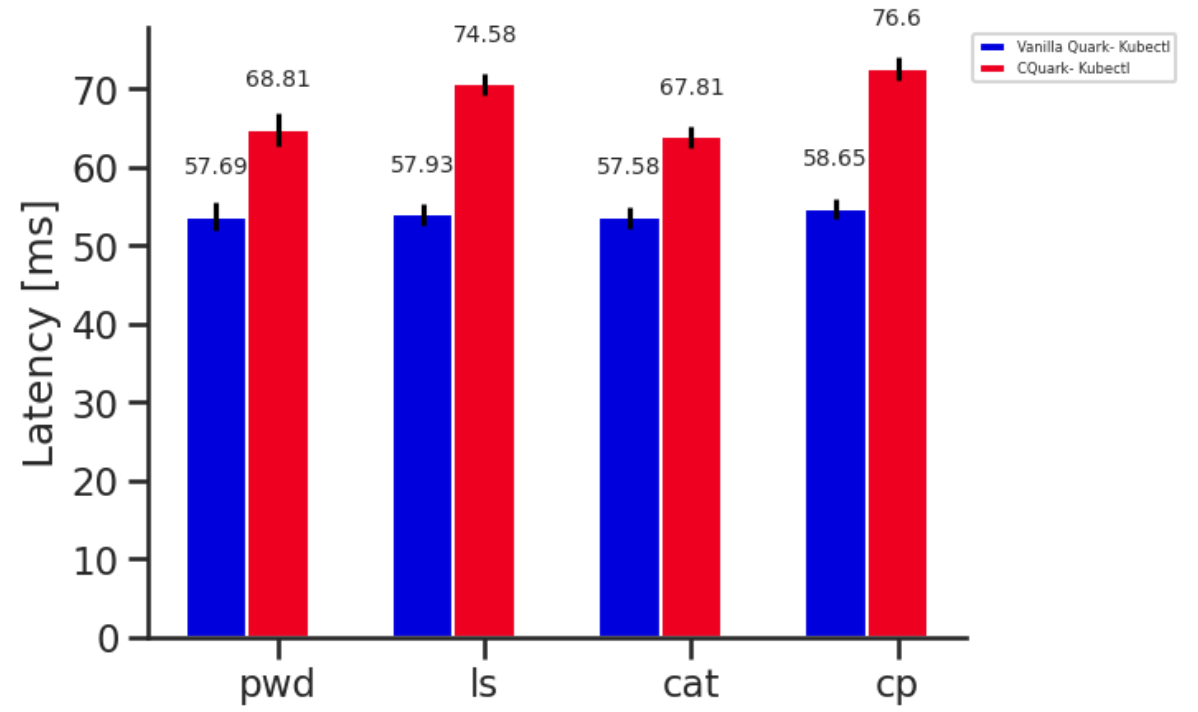
\includegraphics[width=0.9\textwidth]{images/speed_of_issuing_cmd_in_cquark_upstream_quark.PNG} % first figure itself
%         \caption{Benchmark Deployment for testing Speed of accessing file type Secrets in upstream Quark}
%         \label{fig:speed_of_issuing_cmd_in_cquark_upstream_quark}
%     \end{minipage}\hfill
%     \begin{minipage}{0.45\textwidth}
%         \centering
%         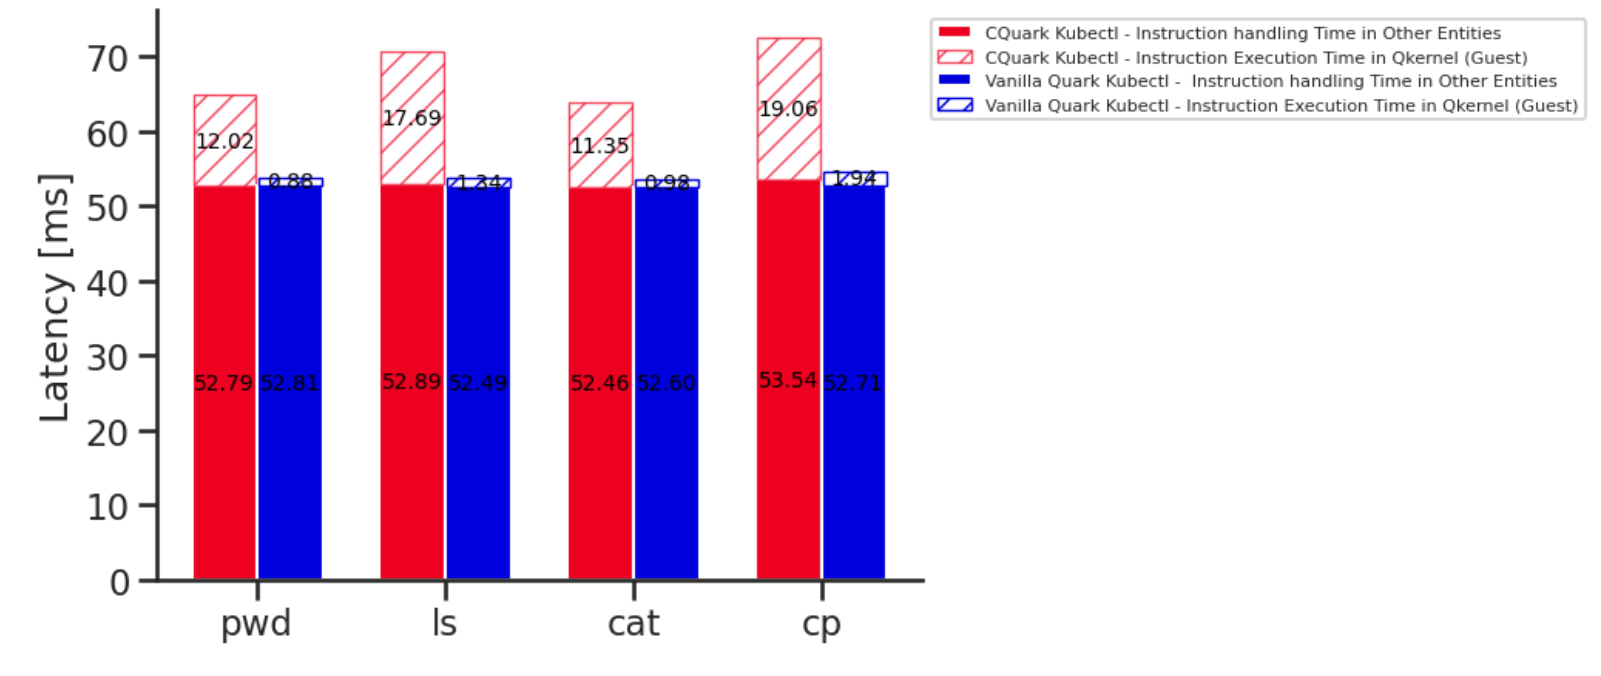
\includegraphics[width=0.9\textwidth]{images/timeshare_issuing_cmd_in_cquark_upstream_quark_kubectl.PNG} % second figure itself
%         \caption{Benchmark Deployment for testing Speed of accessing file type Secrets in confidential Quark}
%         \label{fig:timeshare_issuing_cmd_in_cquark_upstream_quark_kubectl}
%     \end{minipage}
% \end{figure}

\begin{figure}[H]
    \centering
    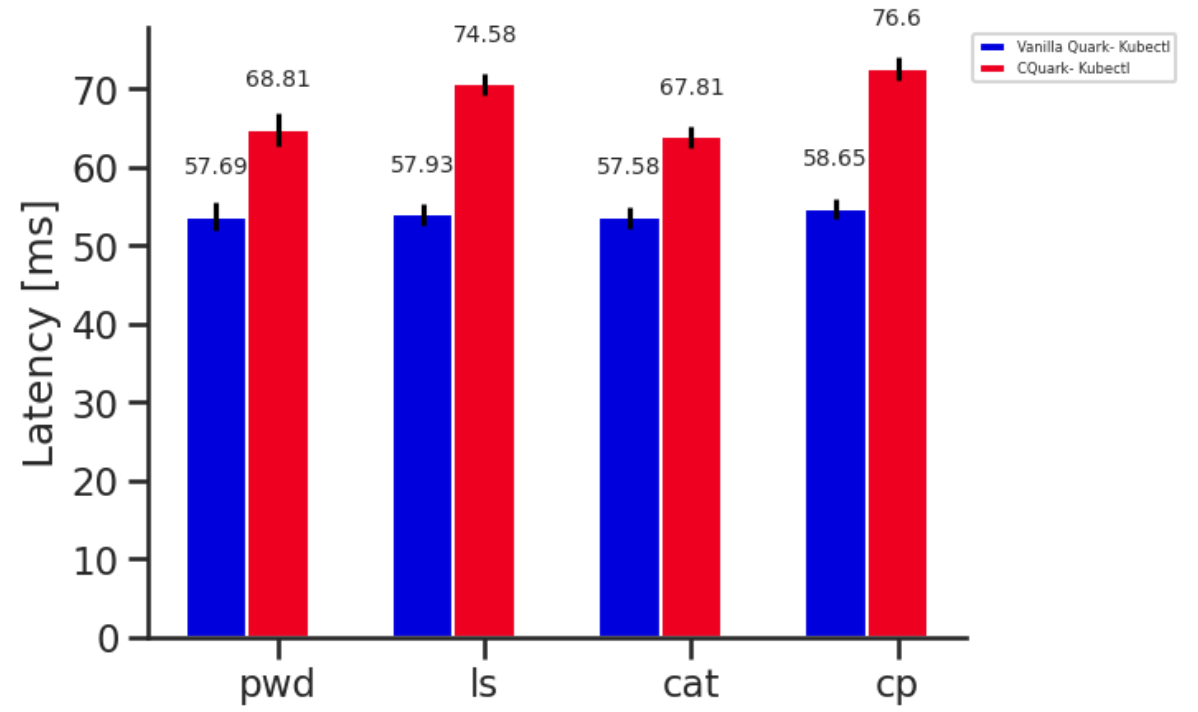
\includegraphics[width=0.8\textwidth]{images/speed_of_issuing_cmd_in_cquark_upstream_quark.PNG}
    \caption[Benchmark result - Latency Comparison of sending Commands to Application in Cquark vs vanilla Quark]{A latency comparison test of sending commands to applications in cquark vs vanilla quark.  The test selects four 
    commonly used Linux commands as samples, each being executed one thousand times. The results indicate that utilizing Kubectl exec to issue instructions to applications in cquark takes over 9\% longer than in vanilla quark.
    }
    \label{fig:speed_of_issuing_cmd_in_cquark_upstream_quark}
\end{figure}




\begin{figure}[H]
    \centering
    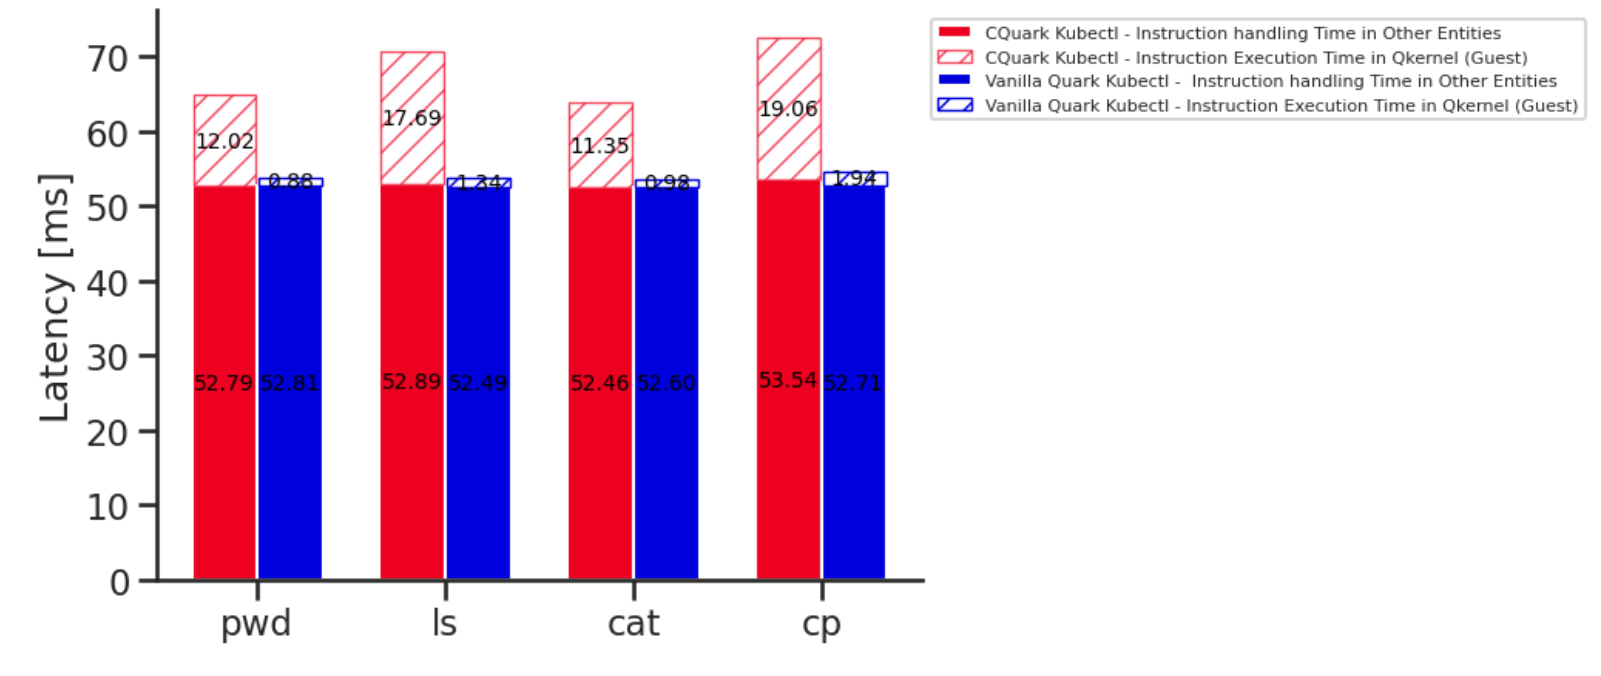
\includegraphics[width=0.8\textwidth]{images/timeshare_issuing_cmd_in_cquark_upstream_quark_kubectl.PNG}
    \caption[Benchmark result - The processing time for each component during the instruction execution lifecycle in confidential vs in vanilla Quark]{Benchmark result of evaluating the percentage of time spent by each component in processing instructions during the instruction execution lifecycle 
    in confidential vs in vanilla Quark . Here the components refer to kubectl,  Kubernetes components for instructions transmission, like containerd, etc., and Qkernel for instruction execution. 
    Each bar in the figure represents the total execution time of an instruction whereby the color-filled section represents the time qkernel used for instruction execution, while the dashed-filled segment implies the time other components took for instruction issuing, transmission, and result handling.
    }
    \label{fig:timeshare_issuing_cmd_in_cquark_upstream_quark_kubectl}
\end{figure}


This section analyses the results illustrated in Figures ~\ref{fig:speed_of_issuing_cmd_in_cquark_upstream_quark} and ~\ref{fig:timeshare_issuing_cmd_in_cquark_upstream_quark_kubectl}. Our finding show that confidential Quark introduces approximately 9\% overhead to the instruction 
execution compared to vanilla quark. This overhead stems from several factors. Firstly, unlike upstream quarks, the Qkernel in Cquark performs authentication and access control for each instruction. Besides, the measurement of the instruction's corresponding binary and guest system call 
interception increases the instruction execution time.  This argument is confirmed in Figure 5.1b, where the average time for Qkernel to execute instructions in vanilla quark is between 1 and 2 ms, while in Cquark, instructions execution in Qkernel takes more than 10 ms. Thus, issuing 
instructions using Kubectl in confidential Quark proves to be more expensive than in vanilla quark.

\begin{figure}[H]
    \centering
    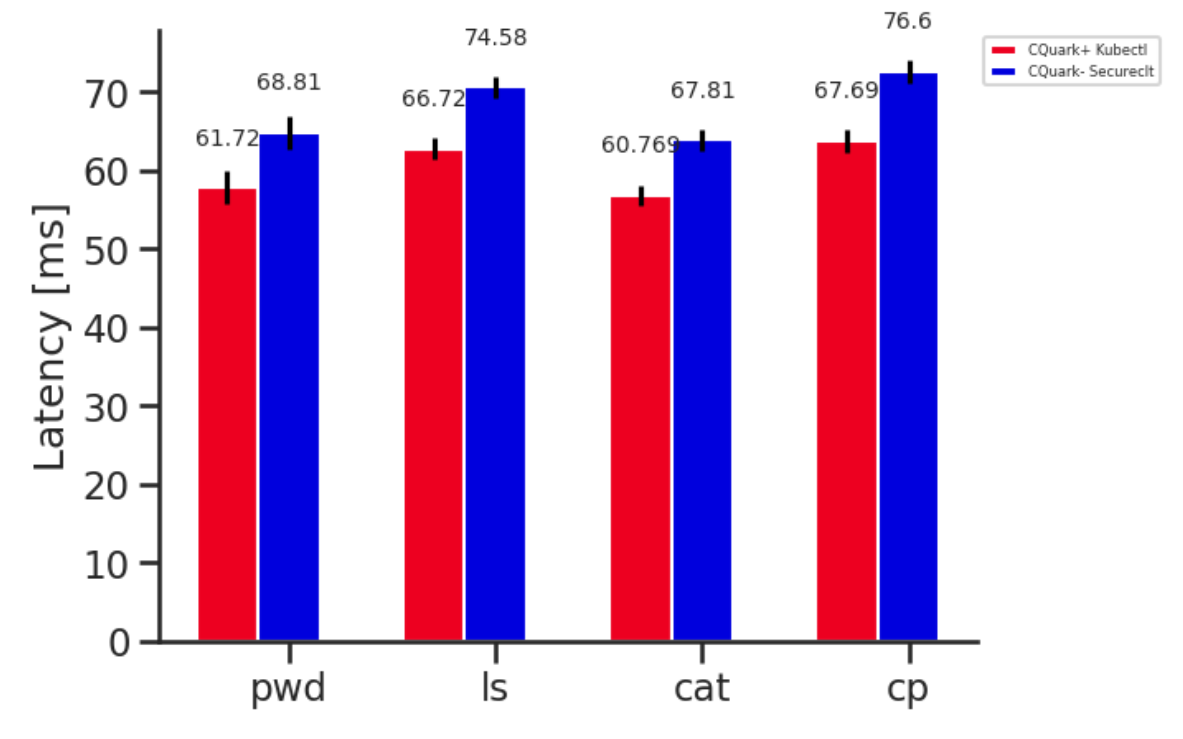
\includegraphics[width=0.8\textwidth]{images/speed_of_issuing_cmd_in_cquark_kubctl_securectl.PNG}
    \caption[Benchmark result - Latency Comparison of issuing privileged instruction vs unprivileged instruction in confidential Quark]{A latency comparison test of issuing privileged instruction vs unprivileged instruction in confidential Quark.  The test included four frequently used Linux 
    commands as samples, each being executed one thousand times.The results indicate that issuing privileged instructions is faster than issuing unprivileged instruction.
    }
    \label{fig:speed_of_issuing_cmd_in_cquark_kubctl_securectl}
\end{figure}


Out of curiosity, we compared the time required to issue privileged and unprivileged instructions in confidential Quark to the application using Securectl and Kubectl, respectively. The results in Figure ~\ref{fig:speed_of_issuing_cmd_in_cquark_kubctl_securectl} reveal that issuing privileged 
instructions is much faster than issuing unprivileged commands. This finding is counterintuitive since privileged instructions require additional cryptographic protection to ensure the confidentiality and integrity of their contents, which implies executing additional code.

\begin{figure}[H]
    \centering
    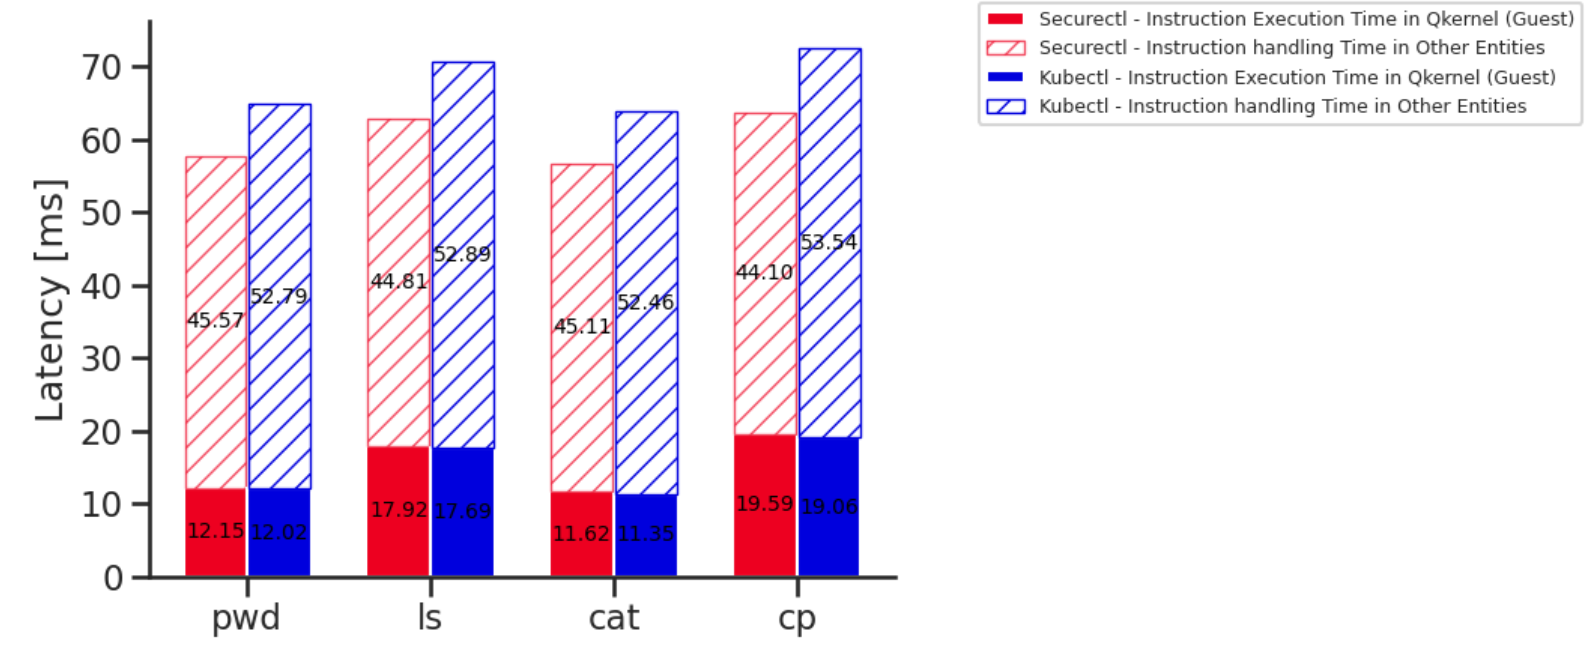
\includegraphics[width=0.8\textwidth]{images/timeshare_issuing_cmd_in_cquark_kubectl_securectl.PNG}
    \caption[Benchmark result - The processing time for components during the privileged vs unprivileged instruction execution lifecycle]{Benchmark result evaluating the percentage of time spent by each component in processing instructions during the privileged versus unprivileged instruction 
    execution lifecycle . Here the components refer to the tool the user employed to issue instructions, i.e., kubectl or securecli,  Kubernetes components for instructions transmission, like containerd, etc., and Qkernel for instruction execution.  Each bar in the 
    figure represents the total execution time of an instruction whereby the color-filled section represents the time qkernel used for instruction execution, while the dashed-filled segment implies the time other components took for instruction issuing, transmission, and result handling.
    }
    \label{fig:timeshare_issuing_cmd_in_cquark_kubectl_securectl}
\end{figure}

To investigate the issue further, we conducted  measurements of processing time for each component during the privileged vs unprivileged instruction execution lifecycle. Here the components refer to the tool the user employed 
to issue instructions, i.e., kubectl or securecli,  Kubernetes components for instructions transmission, like containerd, etc., and Qkernel for instruction execution.
Figure ~\ref{fig:timeshare_issuing_cmd_in_cquark_kubectl_securectl} presents the results obtained. The time incurred by qkernel for executing unprivileged and privileged instructions (color-filled boxes) distinctly shows that the latter takes approximately 0.5 milliseconds more than the former does. 
These latency overheads derive from the decryption and integrity checks that kernel performs for each privileged instruction, as well as the cryptographic protection for the instruction result. However, comparing the time taken by kubectl and securectl to process user requests 
(dashed filled boxes), securectl is significantly faster. Thus, this offsets the cryptographic protection overhead for privileged instructions.

\subsection{Micro-benchmark – Latency Test for accessing binary-mapped memory region}\label{accesiing_binary_mapped_memory}

This section presents the results of a microbenchmark that assesses the speed of accessing binary mapped memory regions during runtime under vanilla and confidential Quark.
% //%or \small or \footnotesize etc.
% \begin{lstlisting}[language=C,frame=single,caption=Program for testing speed of accessing binary-mapped memory region Variant,label=code3,basicstyle=\tiny]
%     #define ARRAY_LEN (unsigned long)(1024*1024*100)    
%     char array[ARRAY_LEN] = {[ 0 ... (1) ] = 'a'} ;

%     int main {
%         struct timespec start, end;
%         clockid_t clk_id = CLOCK_MONOTONIC;  // CLOCK_REALTIME CLOCK_BOOTTIME CLOCK_PROCESS_CPUTIME_ID
%         struct timespec nanos;
%         clock_gettime(CLOCK_MONOTONIC, &nanos);
%         srand(nanos.tv_nsec); 
    
%         for(int i = 0; i < ARRAY_LEN; i++) {
%            index[i] = get_random();
     
%         }
     
%         clock_gettime(clk_id, &start);
%         for(int i = 0; i < ARRAY_LEN; i++) {
%            int current_idx = index[i];
%            //sequential read
%            // char a = array[i];
%            //sequential write
%            // array[i] = 'b';
%            //random read
%            // char a = array[current_idx];
%            //random write
%            // array[current_idx] = 'b';
%         }
%         clock_gettime(clk_id, &end);
     
%         unsigned long long  start_ns = to_ns(start);
%         unsigned long long  end_ns = to_ns(end);
%         printf("start %ju, end  %jun", start_ns, end_ns);

%         return 0;

%     }

 
% \end{lstlisting}

The benchmark utilizes a program\cite*{benchamark_micro} containing a global initialized array located in the binary data segment and a for loop. Within the for loop, the program can access the array by means of four access mode: random read, random write, sequential read, and sequential write. 
We conduct the test in three binary data segment mapped memory sizes, i.e. 5MB, 10MB and 100MB. For each case, the test framework carries out 30 executions of the program in vanilla and confidential Quark in each access mode and calculates the average cost of accessing the array. Note that the size of the binary data 
segment mapped memory region is controlled by the size of the array.


\begin{figure}[ht] 
    \begin{subfigure}[b]{0.5\linewidth}
      \centering
      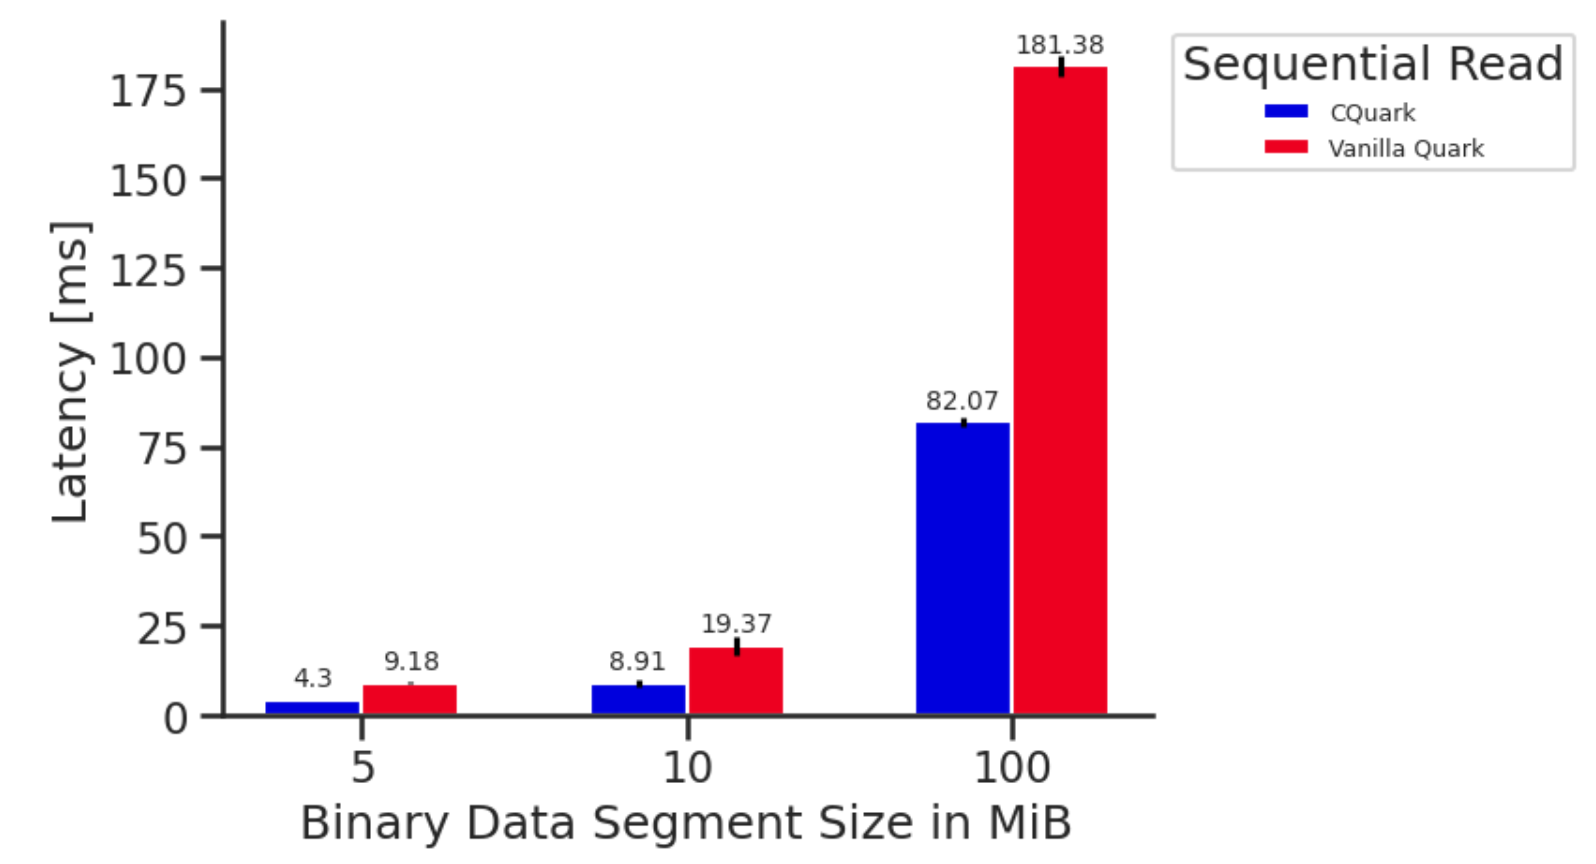
\includegraphics[width=0.9\linewidth]{images/Sequential_Read.PNG} 
      \caption{Sequential Read} 
      \label{fig7:a} 
      \vspace{4ex}
    \end{subfigure}%% 
    \begin{subfigure}[b]{0.5\linewidth}
      \centering
      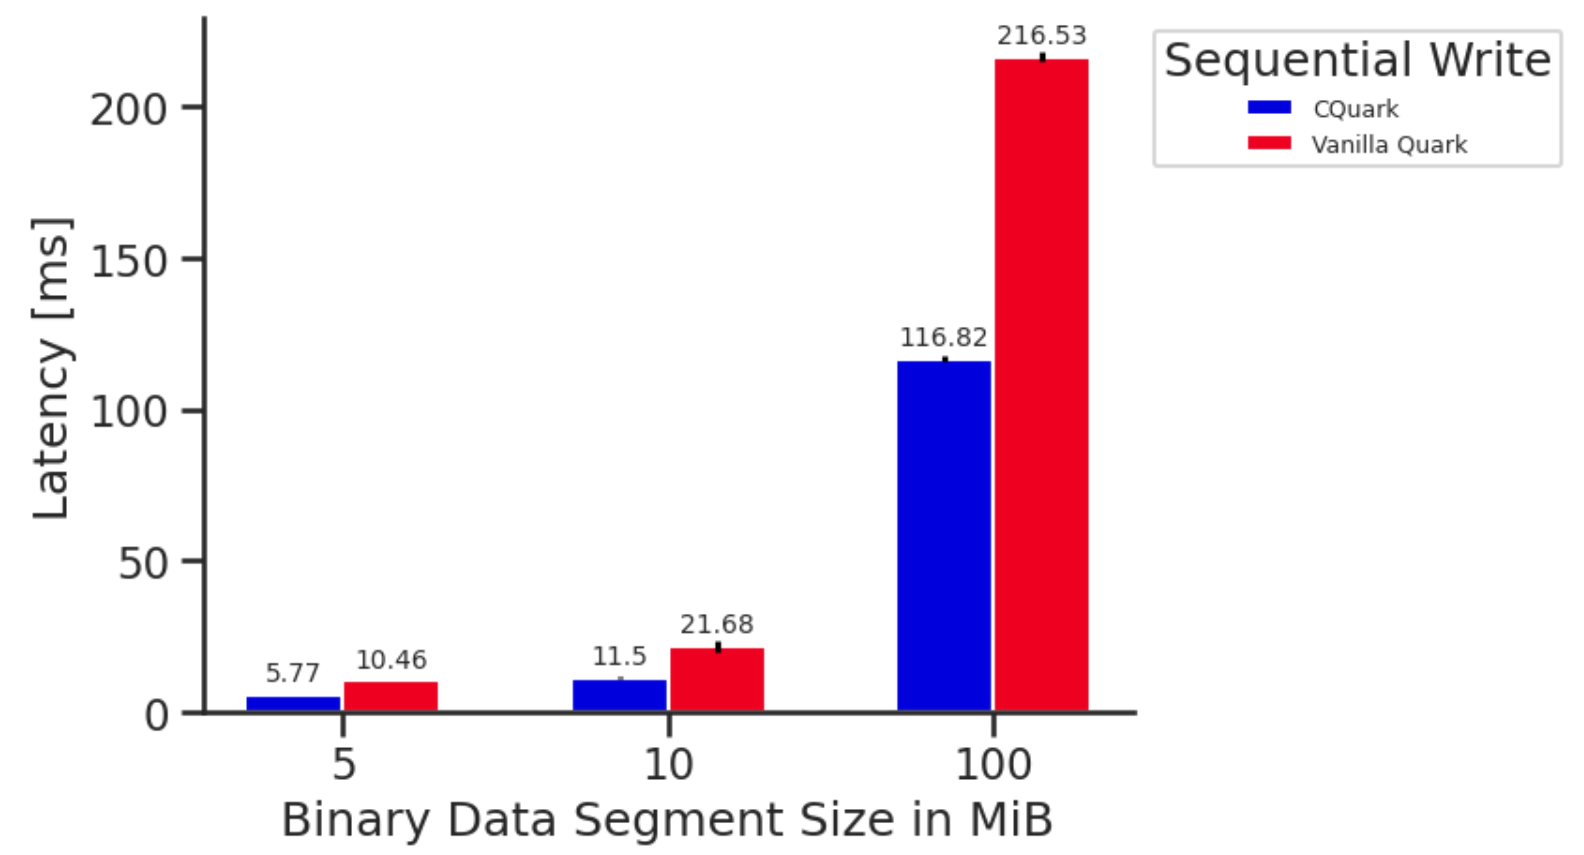
\includegraphics[width=0.9\linewidth]{images/Sequential_Write.PNG} 
      \caption{Sequential Write} 
      \label{fig7:b} 
      \vspace{4ex}
    \end{subfigure} 
    \begin{subfigure}[b]{0.5\linewidth}
      \centering
      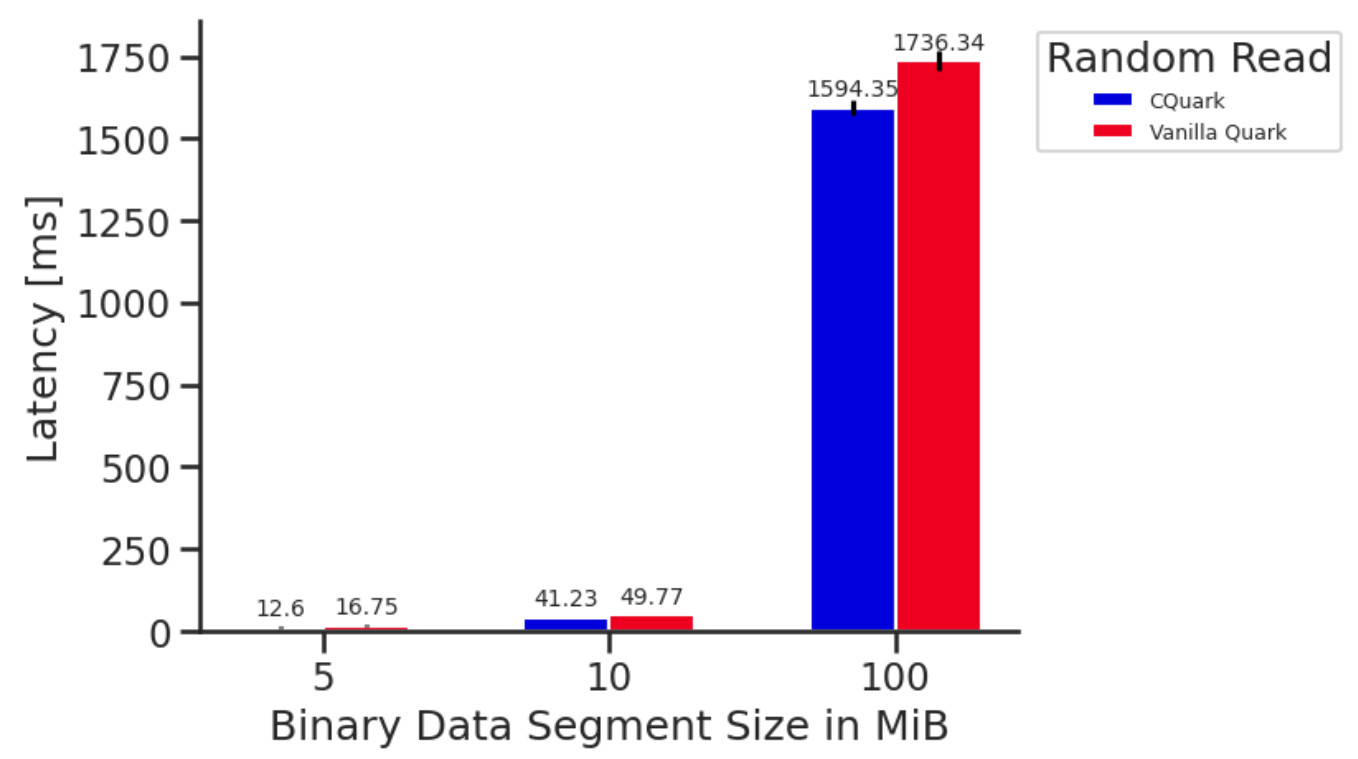
\includegraphics[width=0.9\linewidth]{images/Random_Read.PNG} 
      \caption{Random Read} 
      \label{fig7:c} 
    \end{subfigure}%%
    \begin{subfigure}[b]{0.5\linewidth}
      \centering
      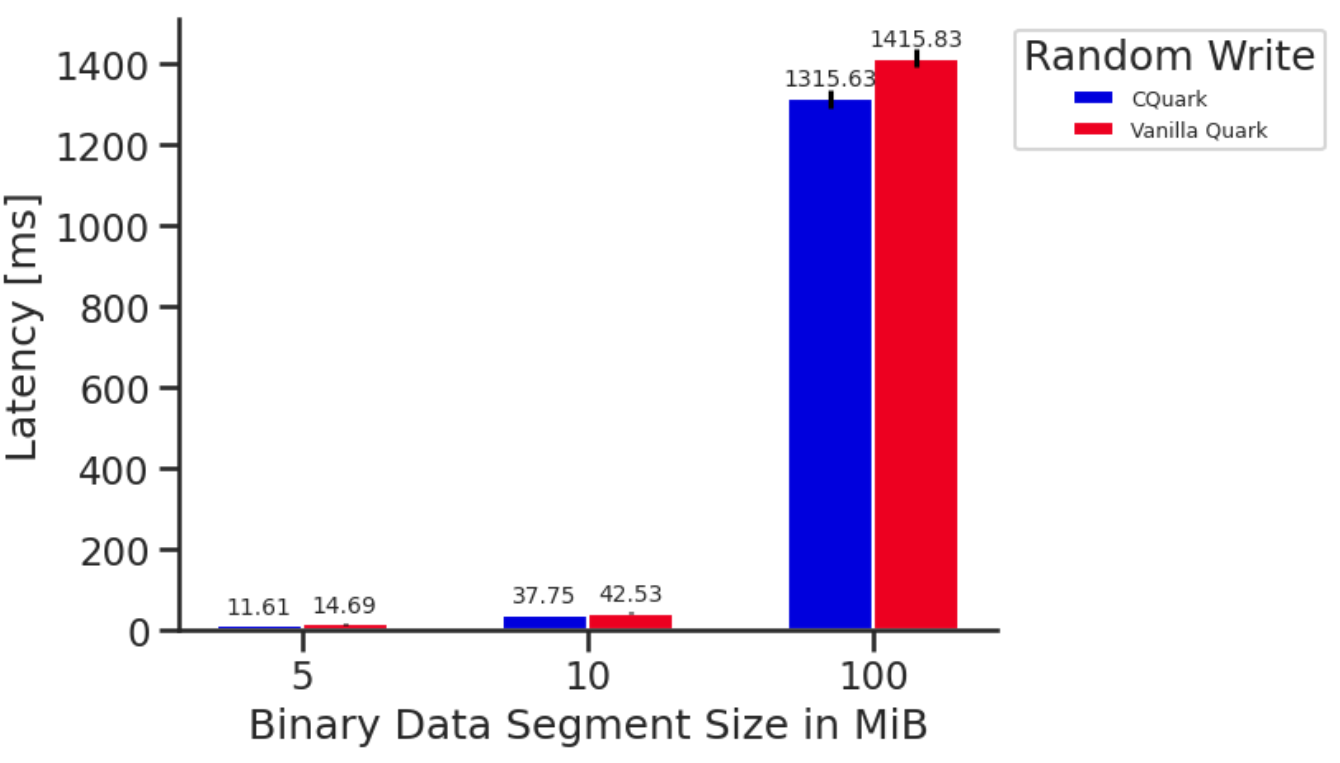
\includegraphics[width=0.9\linewidth]{images/Random_Write.PNG} 
      \caption{Random Write} 
      \label{fig7:d} 
    \end{subfigure} 
    \caption{Benchmark Result - Latency Test for accessing binary-mapped memory region}
    \label{fig7} 
\end{figure}



These results shown in Figure ~\ref{fig7:a} and ~\ref{fig7:b} reveal that confidential Quark improves the performance of sequentially reading and writing binary-mapped memory regions. Specifically, Sequential accessing in confidential Quark is 1.86 times faster than in vanilla quark. This performance 
improvement is due to the fact that measuring binary loaded from host during the program startup prompted qkernel to load the program's binaries from disk into the guest memory. Consequently, the program can access these memory areas at runtime without necessitating page fault handling. 
For the same reason, random reading and writing of binary-mapped memory regions exhibit around 1.08 times faster speed in confidential Quark than in vanilla Quark (Figure ~\ref{fig7:c} and Figure ~\ref{fig7:d}).



\subsection{Micro-benchmark – Latency Test for Application Startup}\label{micro_app_start_up}
The introduction of remote attestation, secret provisioning, and data measurement loaded from the host in confidential Quark results in additional latency overhead for application startup. To examine this overhead, we extended the testing framework to iteratively initiate and terminate the 
application, measuring the start time, exit time, and latency overhead incurred by the remote attestation and provisioning agent, secret injector, hardware evidence driver, and software measurement manager\cite*{benchamark_framework}.

\begin{figure}[H]
    \centering
    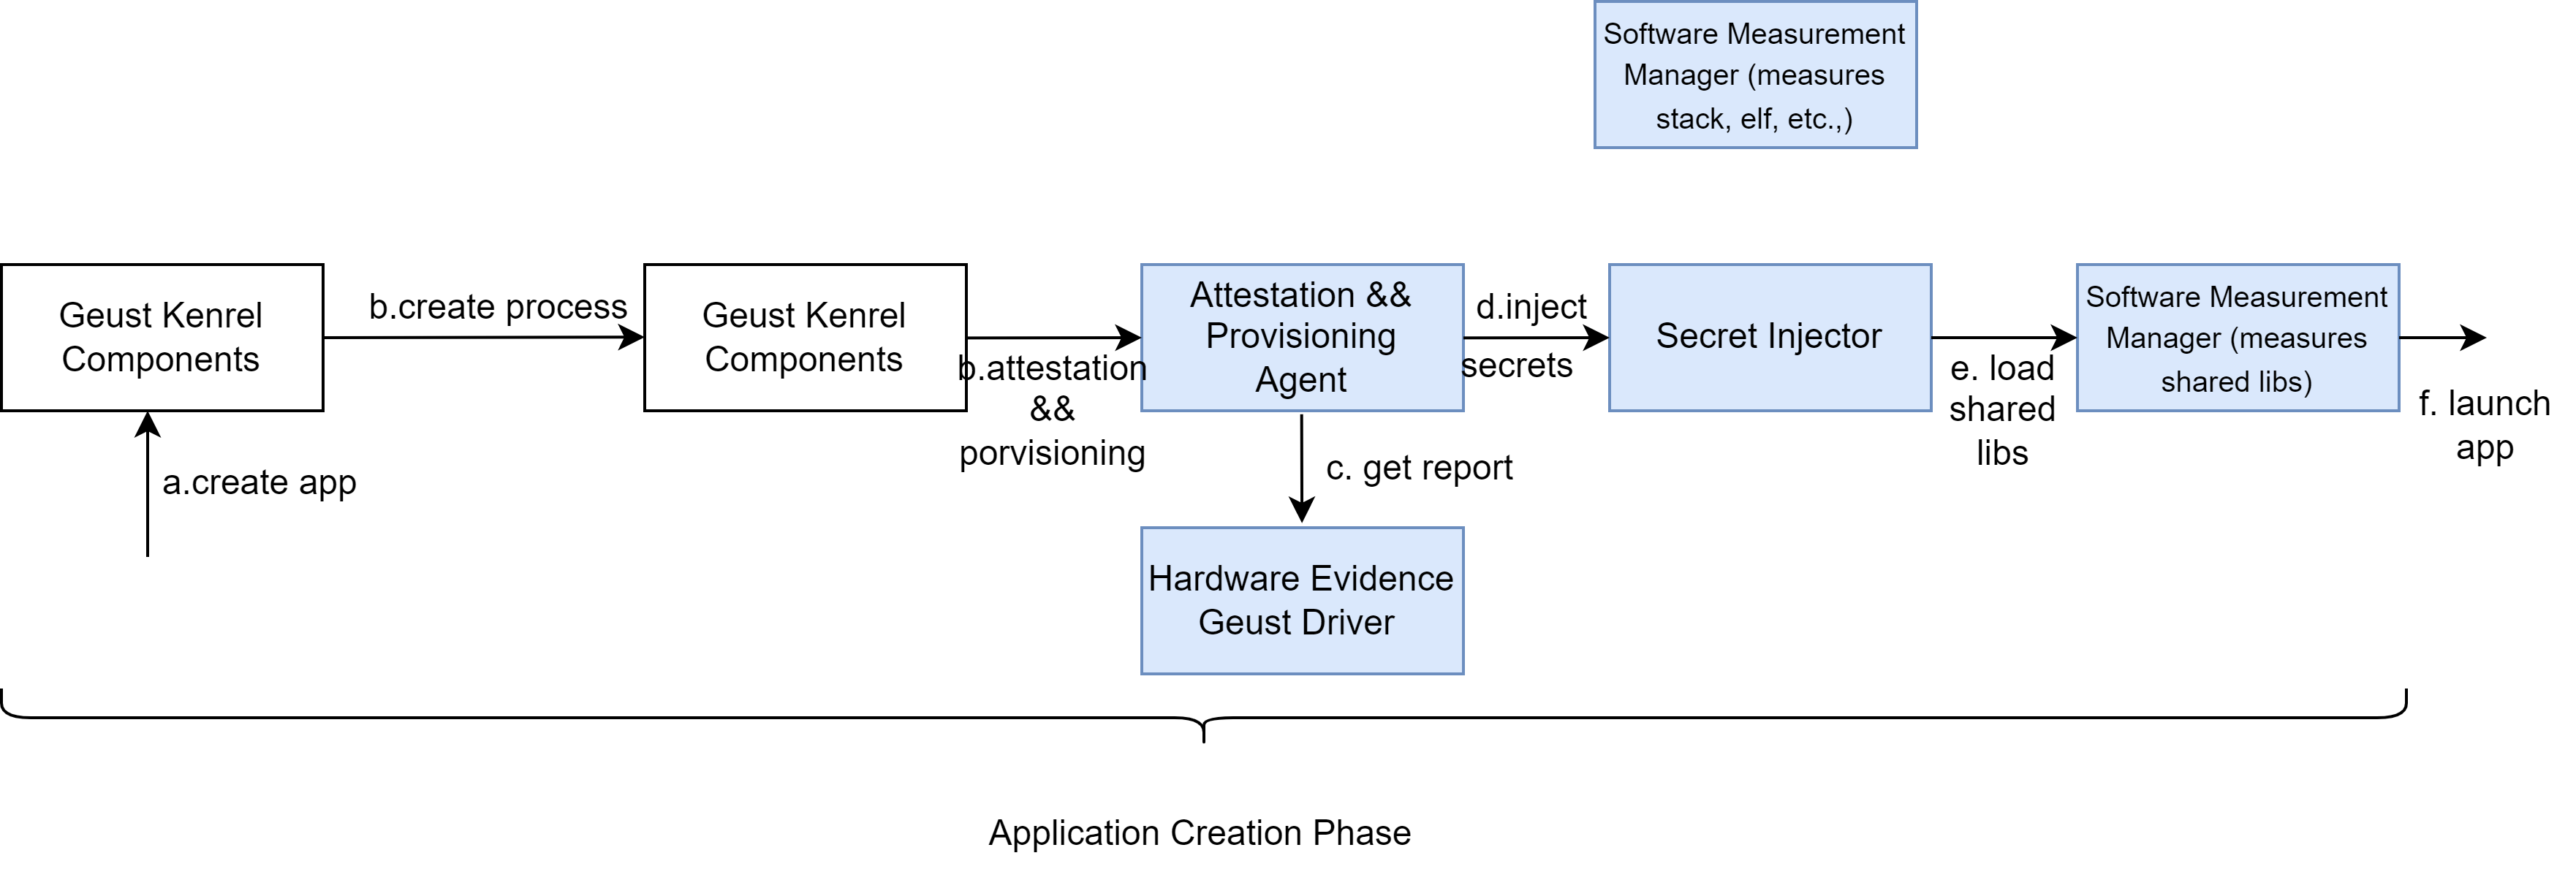
\includegraphics[width=0.8\textwidth]{images/micro_benchmark_app_life_cycle_bencmark_pattern.png}
    \caption[Benchmark Pattern - Latency Test for Application Startup]{Benchmark Pattern - Latency Test for Application Startup}
    \label{fig:micro_benchmark_app_life_cycle_bencmark_pattern}
\end{figure}


Regarding the benchmark methodology. A statically linked hello-world program in Listing ~\ref{code1} is used. To reduce the interference of environmental noise,the test framework runs the application 100 times. In addition, since the remote attestation and provisioning agent, the secret injector, 
the hardware evidence driver, and the software measurement manager shown in Figure  ~\ref{fig:micro_benchmark_app_life_cycle_bencmark_pattern}  (colored boxes) are located in the guest kernel, the test framework cannot directly measure the time spent by these components. Therefore, we use guest clock\_gettime(monotonic)\cite*{clock_gettime} to 
record the time and print the latency overhead of each component to the host using the qkernel logging system. The same approach applies to record the size of data measured by the software measurement manager. 

\begin{lstlisting}[language=C,frame=single,caption=Hello World Program,label=code1]
int main() {
    printf("Hello, World!\n");
    return 0;
}
\end{lstlisting}


As expounded in Chapter 4, two factors may impact the application startup time in confidential Quark: the number of file type secrets and the size of the data measured by the software measurement manager. Hence, this section conducts following three tests. First, we establish a baseline by setting the 
number of file-type secrets to zero and running the hello world program. The test framework measures the program startup time, and records the latency overhead from the remote attestation and provisioning agent, the secret injector, the hardware evidence driver, and the software measurement manager。  
In Experiment 2, we increase the number of file type secrets in order to observe the change in program startup time, as well as the latency overhead from the remote attestation and provisioning agent and the secret injector. In Experiment 3, we examine the growth in the latency overhead of the software 
measurement manager during program startup as the amount of measured data increased. To conduct the test, we utilize a variant of the hello-world program as shown in Listing ~\ref{code2}, incorporating a global initialization array to regulate the data segment size in the binary and thus modify the size 
of software manager measured data during program startup.

\begin{lstlisting}[language=C,frame=single,caption=Hello World Program Variant,label=code2]
#define ARRAY_LEN (unsigned long)(1024*1024*100)    
char array[ARRAY_LEN] = {[ 0 ... (1) ] = 'a'} ;
int main() {     
    printf("Hello, World!\n");
    return 0;
}
\end{lstlisting}


\subsubsection{Creating a Baseline}

This benchmark measures the hello world program's startup time, and the latency overhead caused by remote attestation and provisioning agent, the secret injector, the hardware evidence driver, and the software measurement manager. Note that here the number of file type secrets is 0.

\begin{figure}[H]
    \centering
    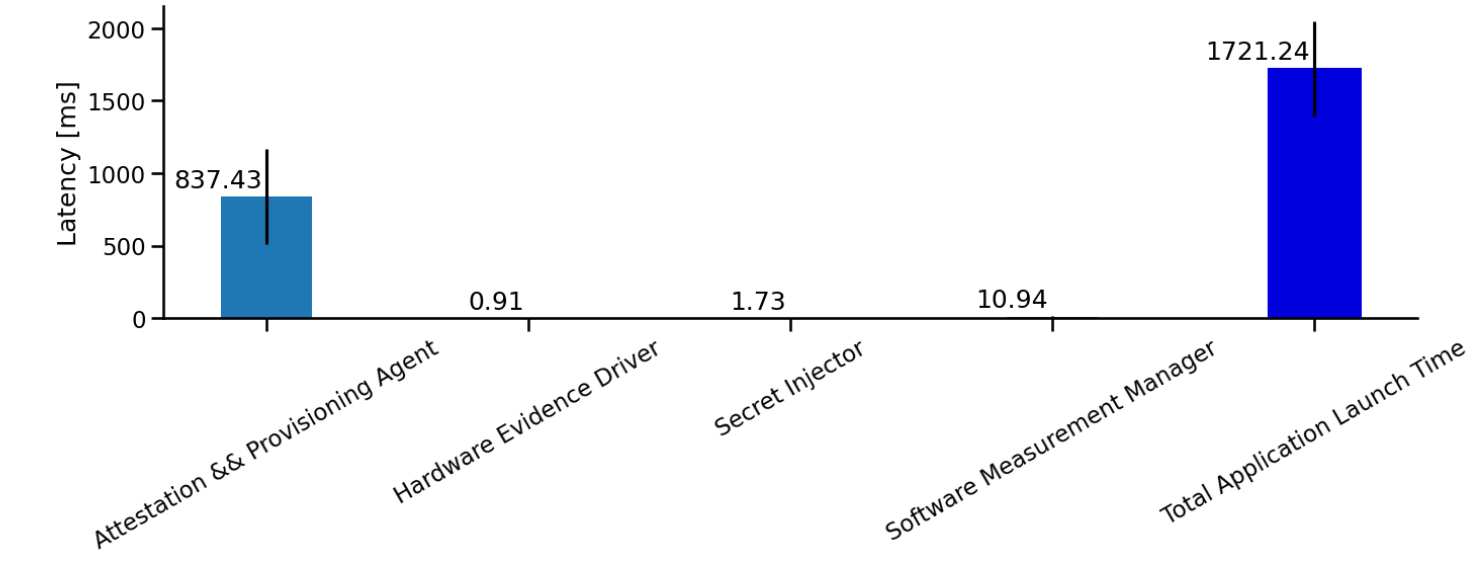
\includegraphics[width=0.8\textwidth]{images/application_start_microtest_baseline_time_overhead_each_cmp.PNG}
    \caption[Benchmark results: Latency Overhead introduce by new Componnents in Cquark]{Benchmark results: Latency Overhead introduce by new Componnents in Cquark}
    \label{fig:application_start_microtest_baseline_time_overhead_each_cmp}
\end{figure}

\begin{figure}[H]
    \centering
    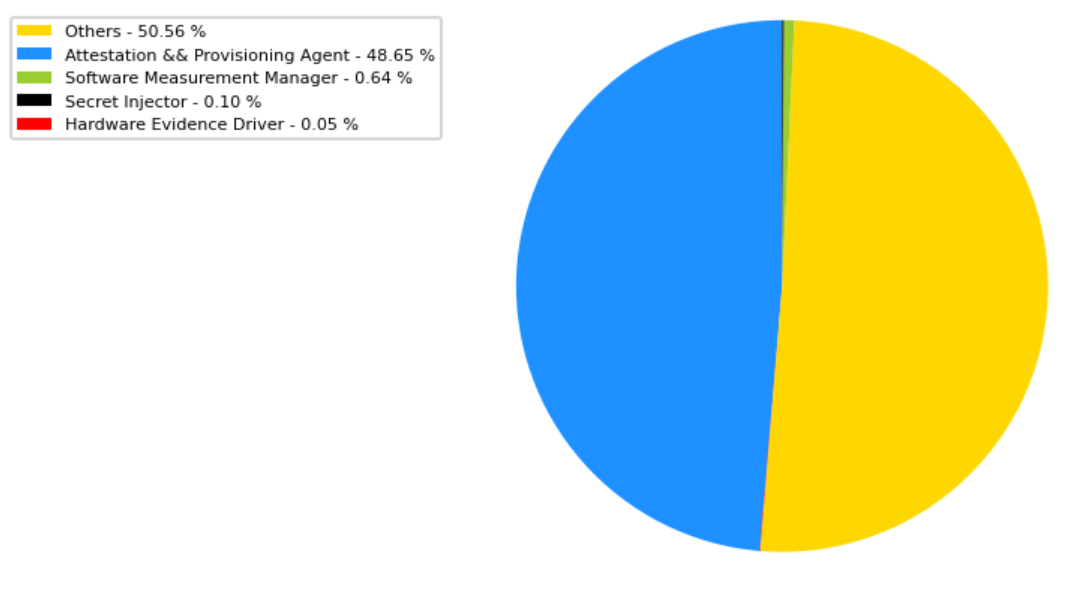
\includegraphics[width=0.8\textwidth]{images/application_start_microtest_baseline_time_distribution.PNG}
    \caption[Time  Distribution of the application startup ]{Distribution of the time consumed by different components in the application startup}
    \label{fig:application_start_microtest_baseline_time_distribution}
\end{figure}



The benchmark results in figure ~\ref{fig:application_start_microtest_baseline_time_overhead_each_cmp} and ~\ref{fig:application_start_microtest_baseline_time_distribution} shows that the remote attestation and provisioning agent, the secret injector, the hardware evidence driver, 
and the software measurement manager doubled the program startup time. Notably, the remote attestation and provisioning agent contributed the most to the latency overhead, which is expected, given its necessity to establish the TLS connection with the relying party, complete the remote 
attestation process, and fetch the enclave policy following the KBS attestation protocol. With regards to the secret injector, the hardware evidence object driver, which is primarily responsible for loading secrets into the application process and generating a simulated hardware report accordingly,  
exhibited a delay overhead of 0.90 milliseconds and 1.73 milliseconds, respectively. However, this delay is negligible compared to the overhead caused by the remote attestation and provisioning agent (~837 milliseconds).  Furthermore, based on the data presented in 
Table ~\ref{table: Measurement_For_Hello_world}, the software measurement manager is found to measure approximately 1.47 MiB of data during program startup, leading to an overhead of only about 10 milliseconds.


\begin{table}[htbp]
    \centering
    \footnotesize
    \caption{Software measurement manager measured data during application startup\strut}
    \begin{tabularx}{1\textwidth}{@{} l L L L L L L@{}}
    \toprule
        Matrics    & ELF &  Shared Library   & Process Spec    & Guest Kernel Args  & Total Measurement\\
    \midrule

        \vn{Measurement}     &  1.447 MiB    &   0 MiB  &   304 Byte      &25004 Byte  & 1.47`' MiB\\
    \bottomrule
    \end{tabularx}
    \label{table: Measurement_For_Hello_world}
\end{table}



\subsubsection{Determining Attestation \&\& Provisioning Agent and Secret Injector Overhead}
The baseline results confirm that the remote attestation and provisioning agent is a significant source of latency overhead. To this end, this section aims to examine how the latency overhead of the remote attestation and provisioning agent, along with the secret injector, changes as the number 
of file-type secrets increases.

\begin{figure}[H]
    \centering
    \includegraphics[width=0.8\textwidth]{images/overhead_attestation_agent_as_file_num_increasing.PNG}
    \caption[Benchmark result: Latency Overhead from Attestation \&\& Provisioning Agent as the number of file-based secrets increases]{Benchmark result: Latency Overhead from Attestation \&\& Provisioning Agent as the number of file-based secrets increases}
    \label{fig:overhead_attestation_agent_as_file_num_increasing}
\end{figure}

\begin{figure}[H]
    \centering
    \includegraphics[width=0.8\textwidth]{images/overhead_secret_injector_as_file_num_increasing.PNG}
    \caption[Benchmark result: Latency Overhead from Secret Injector as the number of file-based secrets increases]{Benchmark result: Latency Overhead from Secret Injector as the number of file-based secrets increases}
    \label{fig:overhead_secret_injector_as_file_num_increasing}
\end{figure}

% , which reveal the evolution of the overhead introduced by the remote attestation and provisioning agent, and 
% secret injector, as the number of file-type secrets grows.

\todo{ add lable after As discussed in Chapter 5,}
This paragraph discusses the benchmark results in Figure ~\ref{fig:overhead_attestation_agent_as_file_num_increasing} and Figure ~\ref{fig:overhead_secret_injector_as_file_num_increasing}. The results demonstrate that the increase in overhead from the remote attestation and provisioning agent, 
and secret injector, is proportional to the number of file-type secrets. As discussed in Chapter 5, constrained by the maximum TLS record size supported by the embedded\_tls library (16kb), the remote attestation and provisioning 
agent must perform one HTTP get + TLS operation for each file-type secret. For the secret injector, it is evident that as the number of files increases, it needs more time to inject the files into the target location in the application process.  Additionally,
Figure ~\ref{fig:startup_time_change_as_file_type_secret_increasing} reveals that although the overhead from the secret injector increases as the number of file secrets grows, it is negligible compared to the overhead from remote attestation and provisioning agent. Moreover, when the 
number of file-type secrets reaches 128, the overhead associated with the remote attestation and provisioning agents becomes astounding, reaching 4500 ms, accounting for over 70\% of the total program startup time.

\begin{figure}[H]
    \centering
    \includegraphics[width=0.8\textwidth]{images/startup_time_change_as_file_type_secret_increasing.PNG}
    \caption[Distribution of the time consumed by attestation \&\& provisioning agent, secret injector and others in the application startup]{Distribution of the time consumed by attestation \&\& provisioning agent, secret injector and others in the application startup}
    \label{fig:startup_time_change_as_file_type_secret_increasing}
\end{figure}



\subsubsection{Impact of measured Data Size}
This benchmark assesses the changes in the software measurer's latency overhead as the application binary size grows.

\begin{figure}[H]
    \centering
    \includegraphics[width=0.8\textwidth]{images/overhead_software_measurement_manager_as_elf_size_increasing.PNG}
    \caption[Benchmark result: Latency Overhead from Software Measurement Manager as the measured Data Size increases]{Benchmark result: Latency Overhead from Software Measurement Manager as the measured Data Size increases}
    \label{fig:overhead_software_measurement_manager_as_elf_size_increasing}
\end{figure}

\begin{figure}[H]
    \centering
    \includegraphics[width=0.8\textwidth]{images/startup_time_change_as_elf_size_increasing.PNG}
    \caption[Distribution of the time consumed by Attestation \&\& Provisioning Agent, Software Measurement Manager and others in the Application Startup]{Distribution of the time consumed by Attestation \&\& Provisioning Agent, Software Measurement Manager and others in the Application Startup}
    \label{fig:startup_time_change_as_elf_size_increasing}
\end{figure}



The benchmark results are in Figure ~\ref{fig:overhead_software_measurement_manager_as_elf_size_increasing}, which shows the latency overhead of the software measurer is proportional to the binary file size, i.e., the more data to be measured, the higher the overhead introduced by the 
software measurer. Furthermore, it is worth mentioning that when measured data less than or equal to 100 MiB, the latency overhead of the software measurer is lower than the overhead introduced by the remote attestation and provisioning agent. 
(Figure ~\ref{fig:startup_time_change_as_elf_size_increasing}).



\subsection{Macro-Benchmark– Application Life Cycle Performance Benchmark}\label{macri_app_start_up}

To evaluate the performance of confidential Quark in a real-world scenario, we conducted the following macro benchmark. The test compares the startup time, exit time, and runtime throughput of real-world applications in confidential and vanilla Quark using Nginx\cite*{nginx} and Redis\cite*{redis}. It should be noted that 
program startup time is measured from the start of the Qkernel to the completion of the dynamic linker (ld.so) loading the application's shared libraries, while the program exit time refers to the time from the time the exit system call is called until qkernel stops running. 
Regarding the application runtime throughput, we use the Apache HTTP server benchmarking tool (AB)\cite*{ab} and Redis-benchmark\cite*{Redis_benchmark} to generate workloads for Nginx and Redis, respectively


Regarding the benchmark methodology and setup, our testing framework\cite*{benchamark_framework} was extended to launch the target application repeatedly, record its startup and exit times, and results from AB\cite*{ab} and Redis-benchmark\cite*{Redis_benchmark}. Specifically, the test framework launches the 
target application 100 times, with the remote attestation and provisioning agent only fetching the shield policy from the relying party. For workload generator’s configuration, Redis benchmark\cite*{Redis_benchmark} and AB\cite*{ab} are set to issue 1,000,000 requests using 50 concurrent clients to Redis and Nginx, respectively. 
In addition, the size of the file requested by ab from Nginx\cite*{nginx} is 181 bytes.

\begin{figure}[H]
    \centering
    \includegraphics[width=0.8\textwidth]{images/reds_nginx_startup_comp.PNG}
    \caption[Redis \&\& Nginx Startup Time in Cquark vs vanilla Quark]{Redis \&\& Nginx Startup Time in confidential vs vanilla Quark}
    \label{fig:reds_nginx_startup_comp}
\end{figure}

The results presented in Figure ~\ref{fig:reds_nginx_startup_comp} indicate that confidential Quark takes about twice as long as vanilla quark to complete the application setup. This result is reasonable, given that Qkernel in Cquark must perform additional operations like remote attestation, 
secret provisioning, and host loaded data measurement, which prolongs the startup time of an application. When comparing the startup time of Nginx and Redis in the Cquark(~\ref{fig:reds_nginx_startup_comp}), we observed that Nginx takes approximately  324 ms longer than Redis to start. 
Since both applications only fetch the shield policy during startup, the latency overhead from the remote attestation and provisioning agent should be identical for both. Therefore, we deduce that the longer Nginx startup time is due to the software measurement manager measuring more data,
resulting in an increased startup time.

\begin{figure}[H]
    \centering
    \includegraphics[width=0.8\textwidth]{images/time_disribution_startup_redis_nginx.PNG}
    \caption[Redis \&\& Nginx  Startup Time in Cquark vs vanilla Quark]{Redis \&\& Nginx  Startup Time in Cquark vs vanilla Quark}
    \label{fig:time_disribution_startup_redis_nginx}
\end{figure}


\begin{table}[htbp]
    \centering
    \footnotesize

    \begin{tabularx}{1\textwidth}{@{} l L L L L L L@{}}
    \toprule
        Matrics    & ELF &  Shared Library   & Process Spec     & Guest Kernel Args  & Total Measurement\\
    \midrule

        \vn{Measurement for Redis}     &  3.64 MiB   &   12.61 MiB  &   304 Byte   &25004 Byte  & 16.27 MiB\\
        \vn{Measurement for Nginx}     &  5.5 MiB    &   61.64 MiB  &   304 Byte   &25004 Byte  & 67.16 MiB\\
    \bottomrule
    \end{tabularx}
    \caption{Software Measurement Manager measured Data during Application Startup\strut}
    \label{table: Measurement_For_Nginx_Redis}
\end{table}


To validate our hypothesis, we measured the overhead induced by the remote attestation and provisioning agent, the secret injector, the hardware evidence driver, and the software measurement manager, as well as the size of the data measured by the software measurer during the application 
startup in confidential Quark. The relevant details can be found in Figure  ~\ref{fig:time_disribution_startup_redis_nginx} and Table ~\ref{table:Measurement_For_Nginx_Redis}. Our findings show that the software measurer measured 16.27 MiB and 67.16 MiB of data for Redis and Nginx respectively, 
leading to a latency of 60.69 ms and 324 ms. Additionally, even though both applications have the same setup for the remote attestation and provisioning agent, the difference in latency overhead from the remote attestation and provisioning agent due to possible network transmission jitter 
was approximately 65 ms. Moreover, the latency generated from the hardware evidence driver and secret injection was less than 1 ms in both cases, which was insignificant compared to the software measurer and remote attestation and provisioning agent's overhead. To summarize, 
Nginx's startup time is longer compared to Redis due to two key reasons - network jitter and Nginx requires the software measurement manager to process more data during setup.

\begin{figure}[H]
    \centering
    \includegraphics[width=0.8\textwidth]{images/reds_nginx_exit_comp.PNG}
    \caption[Redis \&\& Nginx Exit Time in Cquark vs vanilla Quark]{Redis \&\& Nginx Exit Time in Cquark vs vanilla Quark}
    \label{fig:reds_nginx_exit_comp}
\end{figure}


With respect to the application (sandbox) exit, Figure ~\ref{fig:reds_nginx_exit_comp}  shows that confidential Quark can achieves the same performance as vanilla Quark. Specifically, in both confidential and vanilla Quark, the exit time of Redis and Nginx is around 2529 ms.

\begin{figure}[H]
    \centering
    \includegraphics[width=1\textwidth]{images/redis_throughput.PNG}
    \caption[Redis Throughout Test]{Redis Throughout Test Result}
    \label{fig:redis_throughput}
\end{figure}


\begin{figure}[H]
    \centering
    \includegraphics[width=1\textwidth]{images/nginx_throughput.PNG}
    \caption[Nginx Throughout Test]{Nginx Throughout Test Result}
    \label{fig:nginx_throughput}
\end{figure}


The throughput test results for Redis\cite*{redis} and Nginx\cite*{nginx} can be found in Figures ~\ref{fig:redis_throughput} and  ~\ref{fig:nginx_throughput}, respectively. Our analysis shows that execution of Redis and Nginx in confidential Quark led to a performance degradation of 
approximately 22\% and 10\%, respectively. The primary reason for this effect is the interception of the guest system calls.



\subsection{Trust Computing Base}\label{tcb}

In VM-based Trusted Execution Environments (TEE), the Trusted Computing Base (TCB) comprises the necessary hardware, firmware, and software modules, like the guest operating system, that ensure the required security guarantee while handling confidential data. The smaller the TCB, the lower the 
risk of a TEE being compromised by a vulnerability. Therefore, in this section, we evaluate the TCB overhead introduced by our implementation and compares the TCB size between confidential Quark and Confidential Container\cite*{confidential_kata}. To assess confidential Quark-incurred TCB overhead, 
we compare the lines of code and the size of the guest kernel binary in confidential and vanilla Quark as both use a application kernel as the guest kernel and the shield layer is part of  the guest kernel binary.  For the TCB size comparison between confidential Quark and the Confidential Container\cite*{confidential_kata}, 
we use the binary size of the Guest assets as a reference.  To ensure fairness, we employ the strip utility\cite*{strip} to remove unused symbols in binaries.

\begin{table}[htbp]
    \centering
\begin{tabular}{lrrrcrrr}\toprule
    \hline
    \multicolumn{3}{c}{Vanilla Quark}&&\multicolumn{3}{c}{Confidential Quark}\\
    \cline{1-3}\cline{5-7}
    $Component$ & $LoC$ & $Size$$^{3}$ && $Component$ & $LoC$ & $Size$$^{3}$\\
  \midrule
     Qkernel &32487 & -&& Qkernel&32487&-\\
     Qlib &85128  & -&&Qlib&  86609 &-\\
     Shield  & 0 & - && Shield&2805&-\\
  
     \midrule
      Total  & 117615& 3.1MiB&& & 121901 &  4.6 MiB\\
      \bottomrule
  \end{tabular}

  \caption{Comparison of the LoC and compiled size of vanilla quark and confidential quark\strut}
  \label{table:tcb_size_quark_vs_cquark}
\end{table}

Table ~\ref{table:tcb_size_quark_vs_cquark} provides a summary of the TCB overhead required to achieve confidentiality in confidential Quark. The vanilla Quark version v2.0 has a guest kernel with 11,7615 lines of code and generates a 3.10 MB static linked binary. In confidential Quark, our implementation adds 4286 LoC to the guest binary, 
bringing the total to 12,1901 LoC and 4.6 MB of compiled static linked binary. Overall, our implementation makes the guest binary 1.48 times larger compared to vanilla Quark.


\begin{table}[htbp]
    \centering
\begin{tabular}{lrrcrr}\toprule
    \hline
    \multicolumn{2}{c}{Confidential Container}&&\multicolumn{2}{c}{Confidential Quark}\\
    \cline{1-2}\cline{4-5}
    $Component$  & $Size$$^{3}$ && $Component$  & $Size$$^{3}$\\
  \midrule
     Guest Kernel &47.16 MiB && Guest kernel &4.6 MiB\\
     OVMF   & 4 MiB && &   &\\
     Kata agent  & 22.65MiB  && &&\\
  
     \midrule
        & 73.81 MB&& &   4.6 MiB\\
      \bottomrule
  \end{tabular}

  \caption{TCB size comparison between confidential container vs confidential quark in terms of compiled size of guest assets \strut}
  \label{table:tcb_size_quark_vs_kata}
\end{table}

Table ~\ref{table:tcb_size_quark_vs_kata} shows the outcomes of comparing the TCB size in the Confidential Container (Kata)\cite*{confidential_kata} and confidential Quark. Unlike confidential Quark, which uses the application kernel as the guest kernel, Confidential Container deploys 
the qemu-linux base virtual machine. Therefore, the guest assets in the Confidential Container context include the Kata agent\cite*{kata_agent}, OVMF\cite*{ovmf}, and Linux Guest kernel. In the Confidential Container version v0.4, the compiled static binary sizes of Kata agent, OVMF, and Guest kernel are 22.65 Mb, 4.0 MB, and 47.16 MB, 
respectively. This totals a TCB size of 73.81 MB, which is about 16 times greater than that of confidential Quark.

It is noteworthy that there is potential to further optimize the size of Quark's Trusted Computing Base (TCB).  In Quarkv version 2.0, qlib contributes some redundant code to guest kernel binary. To facilitate code development, the qlib code is shared between qvisor and guest kernel. 
However, our founding shows some code in qlib is only used by functions in qvisor, thus increasing the size of the guest kernel’s binary. 

\section{Summary}
In this chapter, I conducted both qualitative and quantitative analyses to evaluate my work. In the qualitative analysis, I identified potential security vulnerabilities in vanilla Quark and explained how my work mitigates these vulnerabilities. 
Regarding the quantitative analysis, I developed a testing framework to characterize the performance of CQuark. The obtained results showed that confidential Quark engenders significant overhead compared to vanilla Quark. 
This overhead is visible in longer program creation times, reduced runtime program throughput, reduced speed of issuing instructions to the program, increased trusted computing base (TCB) size, etc.




% \begin{table}[htp]
%     \caption{Software measurement manager measured data during application startup}
%     \begin{tabularx}{\textwidth}{*{2}{p{0.5\textwidth}}}\toprule
%                                  & ELF &  Shared Library   & Process Spec  & Stack   & Guest Kernel Args  & Total Measurement \\ \midrul
%     Measurement For Hello world  &  1.4468 MiB    &   0 MiB  &   3819 Byte   & 305 Byte   &5865 Byte  & 1.457 MiB \\\addlinespace
%     \bottomrule
%     \end{tabular}
%     \label{table: Measurement_For_Hello_world}
% \end{table}


% \begin{table}[!ht]
%     \sffamily
%     \caption{Terminologies in SQL \& corresponding in MongoDB}
%     \label{tab:my_label}
%     \centering
%     \begin{tabularx}{\textwidth}{*{2}{p{0.5\textwidth}}}
%     \toprule
%                                  & ELF &  Shared Library   & Process Spec  & Stack   & Guest Kernel Args  & Total Measurement \\ \midrule
%     Measurement For Hello world  &  1.4468 MiB    &   0 MiB  &   3819 Byte   & 305 Byte   &5865 Byte  & 1.457 MiB \\\addlinespace
%     \dots & \dots \\
%     \bottomrule
%     \end{tabularx}
%     \end{table}




\cleardoublepage

%%% Local Variables:
%%% TeX-master: "diplom"
%%% End:
